\documentclass[10pt,a4paper]{llncs}

\usepackage[utf8x]{inputenc}
\usepackage{url}
\usepackage{graphicx}
\usepackage{amssymb,amsmath}
\usepackage{textcomp}
\usepackage{float}
\usepackage[dvips,a4paper]{geometry}

\usepackage{url}
\usepackage{array}
\RequirePackage[table]{xcolor}% for colored tabular rows 
\usepackage{microtype}% optimized spacing
\usepackage[tight,footnotesize]{subfigure}% subfloats
\geometry{lmargin=30mm,rmargin=30mm,tmargin=30mm,bmargin=30mm}

\title{Human Action Classification in Still Images}
\author{Vincent Delaitre} \institute{%
\email{vincent.delaitre@ens-lyon.fr}
}%
% \keywords{}

\begin{document} 

% ===============================================================================%
\section{$K$-Nearest classifier + Bag-of-features}
%--------------------------------------------------------------------------------%
\subsection{Tested Parameters}

\subsubsection{Detectors}
\begin{itemize}
\item HARRIS(S): Harris-Laplace detector with only scale invariance.
\item HARRIS(SR): Harris-Laplace detector with scale and rotation invariance.
\item DENSE: Dense features.
\item MSDENSE: Multi-scale dense features.
\end{itemize}

\subsubsection{Descriptors}
\begin{itemize}
\item SIFT(L2): SIFT descriptor normalized with L2 norm.
\item SIFT(L2T): SIFT descriptor normalized with L2 norm and truncation over 0.2.
\end{itemize}

\subsubsection{Dictionnary size}$~$\\
Tested sizes: 128, 256, 512, 1024.

\subsubsection{Histogram normalization}
\begin{itemize}
\item NONE: no normalization.
\item L1: normalized with L1 norm.
\item L2: normalized with L2 norm.
\end{itemize}

\subsubsection{Classifier}$~$\\
Classifier is $K$-nearest neighbours with $K$ from 1 to 5.

%--------------------------------------------------------------------------------%
\subsection{Results}


\subsubsection{Detector}$~$\\

\begin{table}[H]
\centering
\caption{KKN+BOF: Average performances for different detectors. The mean is computed over all other combinaison of parameters.}
\label{table:KNN_BOF:Detector}
\begin{tabular}{|l|c|c|c|c|}
\hline
$~~$Detector & HARRIS(S) & HARRIS(SR) & DENSE & MSDENSE \\ \hline
$~~$Avg. perf.$~~$ & $~~36.9 \pm 3.0~~$ & $~~36.9 \pm 2.8~~$ & $~~38.1 \pm 4.0~~$ & $~~\mathbf{40.8 \pm 2.8}~~$ \\ \hline
\end{tabular}
\end{table}

\subsubsection{Descriptor}$~$\\

\begin{table}[H]
\centering
\caption{KKN+BOF: Average performances for different descriptors. The mean is computed over all other combinaison of parameters.}
\label{table:KNN_BOF:Descriptor}
\begin{tabular}{|l|c|c|}
\hline
$~~$Descriptor & SIFT(L2) & SIFT(L2T) \\ \hline
$~~$Avg. perf.$~~$ & $~~\mathbf{38.3 \pm 3.6}~~$ & $~~38.1 \pm 3.5~~$ \\ \hline
\end{tabular}
\end{table}

However, L2T is better for bigger value of K for K-nearest neighbour classification:

\begin{figure}[H]
\centering
\caption{KKN+BOF: Performances for $K \in \{1, \cdots, 5\}$ across different dictionnary size. Left and right graphics are respectively obtained using the L2 and L2T norm.}
\label{fig:KNN_BOF:SIZE_K_graph}
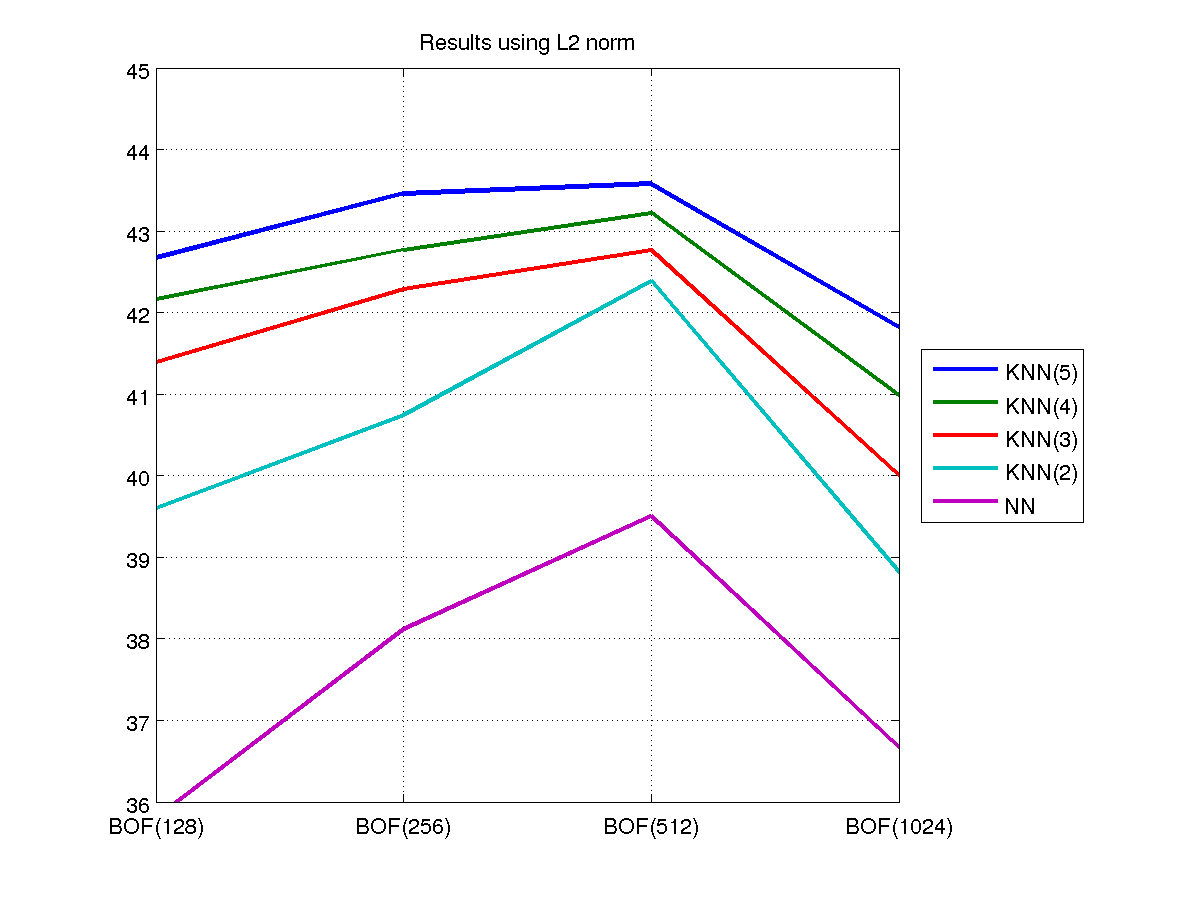
\includegraphics[scale=0.365]{img/KNN_BOF_SIZE_K_graph_L2.png} \hfill
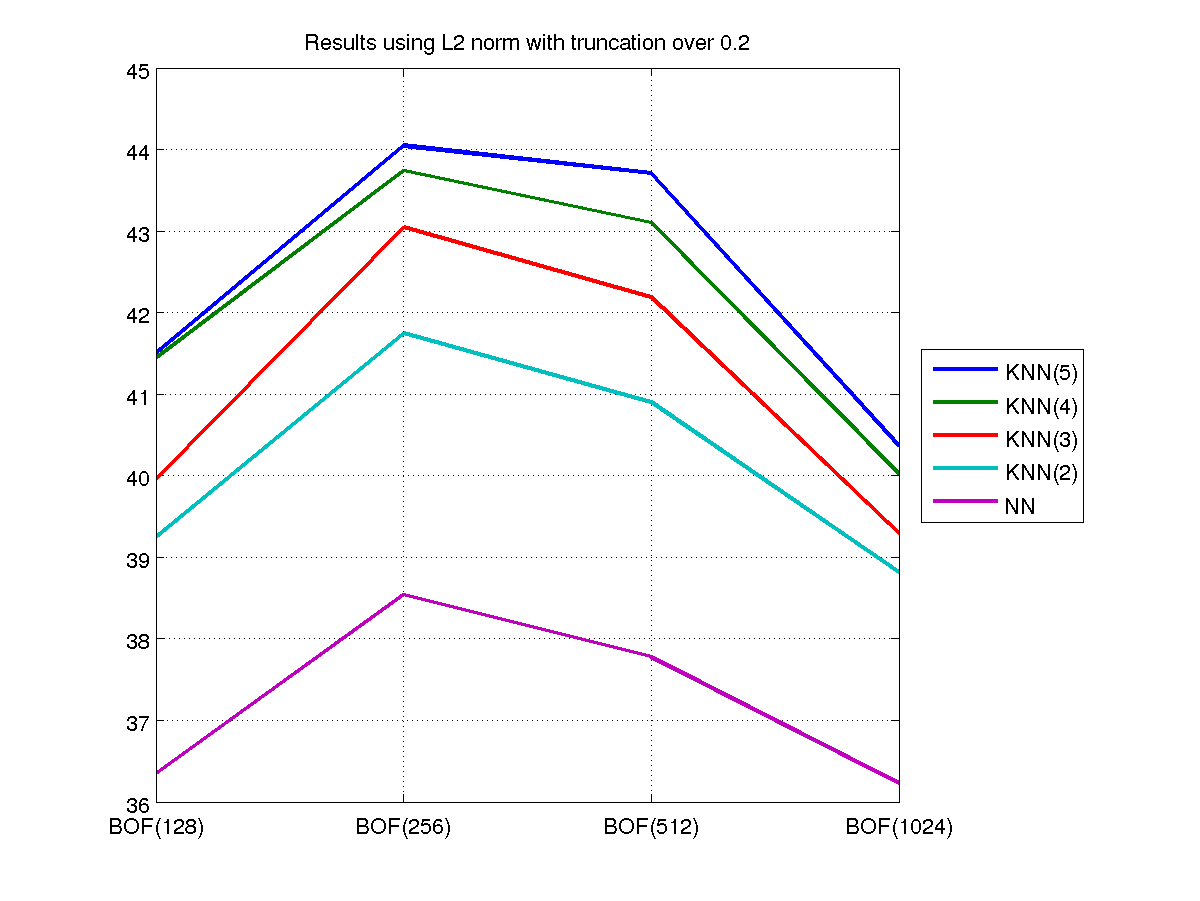
\includegraphics[scale=0.365]{img/KNN_BOF_SIZE_K_graph_L2T.png}
\end{figure}

\subsubsection{Dictionnary size}$~$\\

\begin{table}[H]
\centering
\caption{KKN+BOF: Average performances for different dictionnary size. The mean is computed over all other combinaison of parameters.}
\label{table:KNN_BOF:DicSize}
\begin{tabular}{|l|c|c|c|c|}
\hline
$~~$Dic. Size & 128 & 256 & 512 & 1024 \\ \hline
$~~$Avg. perf.$~~$ & $~~38.0 \pm 3.2~~$ & $~~39.1 \pm 3.0~~$ & $~~\mathbf{39.2 \pm 2.7}~~$ & $~~36.5 \pm 4.4~~$ \\ \hline
\end{tabular}
\end{table}

\subsubsection{Histogram normalization}$~$\\

\begin{table}[H]
\centering
\caption{KKN+BOF: Average performances for different normalization of the signature histogram. The mean is computed over all other combinaison of parameters.}
\label{table:KNN_BOF:Histonorm}
\begin{tabular}{|l|c|c|c|}
\hline
$~~$Histo. Norm & NONE & L1 & L2 \\ \hline
$~~$Avg. perf.$~~$ & $~~37.8 \pm 4.4~~$ & $~~38.1 \pm 3.1~~$ & $~~\mathbf{38.6 \pm 2.9}~~$ \\ \hline
\end{tabular}
\end{table}

However, if we consider only the Multi-scale dense detector, L1 performs better than L2 and NONE norms:

\begin{table}[H]
\centering
\caption{KKN+BOF: Average performances for different normalization of the signature histogram. The detector is MSDENSE and the mean is computed over all other combinaison of parameters.}
\label{table:KNN_BOF:HistonormMSDENSE}
\begin{tabular}{|l|c|c|c|}
\hline
$~~$Histo. Norm & NONE & L1 & L2 \\ \hline
$~~$Avg. perf.$~~$ & $~~40.8 \pm 3.5~~$ & $~~\mathbf{40.9 \pm 2.3}~~$ & $~~40.5 \pm 2.5~~$ \\ \hline
\end{tabular}
\end{table}


\subsubsection{Classifier}$~$\\

\begin{table}[H]
\centering
\caption{KKN+BOF: Average performances for different values of K.}
\label{table:KNN_BOF:Classifier}
\begin{tabular}{|l|c|c|c|c|c|}
\hline
$~~$K & 1 & 2 & 3 & 4 & 5 \\ \hline
$~~$Avg. perf.$~~$ & $~~35.3 \pm 2.9~~$ & $~~37.8 \pm 2.9~~$ & $~~38.8 \pm 3.1~~$ & $~~39.3 \pm 3.4~~$ & $~~\mathbf{39.6 \pm 3.6}~~$ \\ \hline
\end{tabular}
\end{table}

%--------------------------------------------------------------------------------%
\subsection{Accurracy and Precision-Recall}

Classifier: K-Nearest Neighbours (K = 5)\\
Signature: Bag of features (K = 256)\\
Histogram normalization: None\\
K-means library: cpp\\
Channels:\\
(DENSE[spacing = 12-14-17-20-24-29-35-42-51-61, library: mylib]) x (SIFT[normalization: L2 (norm = 1, truncation over 0.2), library: cd])\\

\begin{table}[H]
\centering
\caption{KKN+BOF: Confusion table. The average accurracy is \textbf{42.1\%}.}
\label{table:KNN_BOF:Accuracy}
\rowcolors[]{1}{white}{gray!10}
\begin{tabular}{|l|c|c|c|c|c|c|c|}
\hline
$Actions $ & $~~$(1)$~~$ & $~~$(2)$~~$ & $~~$(3)$~~$ & $~~$(4)$~~$ & $~~$(5)$~~$ & $~~$(6)$~~$ & $~~$(7)$~~$\\ \hline
(1) Interacting With Computer & \cellcolor{lightgray}\textbf{39.47} & 10.53 & 18.42 & 5.26 & 10.53 & 10.53 & 5.26 \\ \hline
(2) Photographing             & 0.00 & 26.32 & 6.58 & 9.21 & 18.42 & 11.84 & \cellcolor{lightgray}\textbf{27.63} \\ \hline
(3) Playing Music             & 6.90 & 24.14 & \cellcolor{lightgray}\textbf{27.59} & 6.90 & 12.07 & 6.03 & 16.38 \\ \hline
(4) Riding Bike               & 0.71 & 8.51 & 5.67 & \cellcolor{lightgray}\textbf{51.06} & 9.93 & 14.18 & 9.93 \\ \hline
(5) Riding Horse              & 5.26 & 17.54 & 8.77 & 3.51 & \cellcolor{lightgray}\textbf{38.60} & 14.04 & 12.28 \\ \hline
(6) Running                   & 1.27 & 7.59 & 3.80 & 5.06 & 8.86 & \cellcolor{lightgray}\textbf{54.43} & 18.99 \\ \hline
(7) Walking                   & 0.00 & 8.40 & 0.00 & 5.04 & 10.92 & 18.49 & \cellcolor{lightgray}\textbf{57.14} \\ \hline
\end{tabular}
\end{table}


\begin{figure}
\caption{KKN+BOF: Precision-Recall. The average precision is \textbf{46.5\%}.}
\label{fig:NN_BOF_PR}
\begin{minipage}{0.5\linewidth}
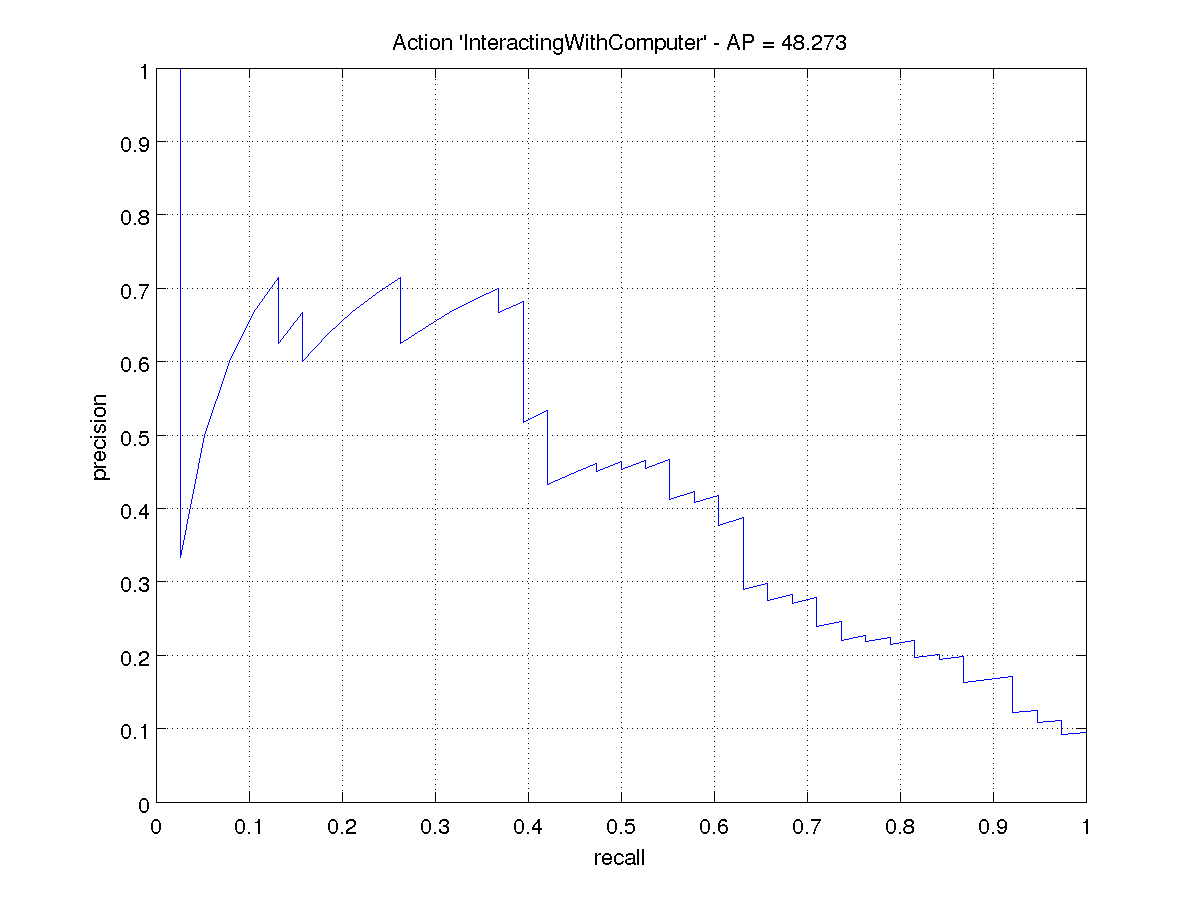
\includegraphics[height=5cm]{img/KNN_BOF_PR_InteractingWithComputer.png}
\end{minipage}
\begin{minipage}{0.5\linewidth}
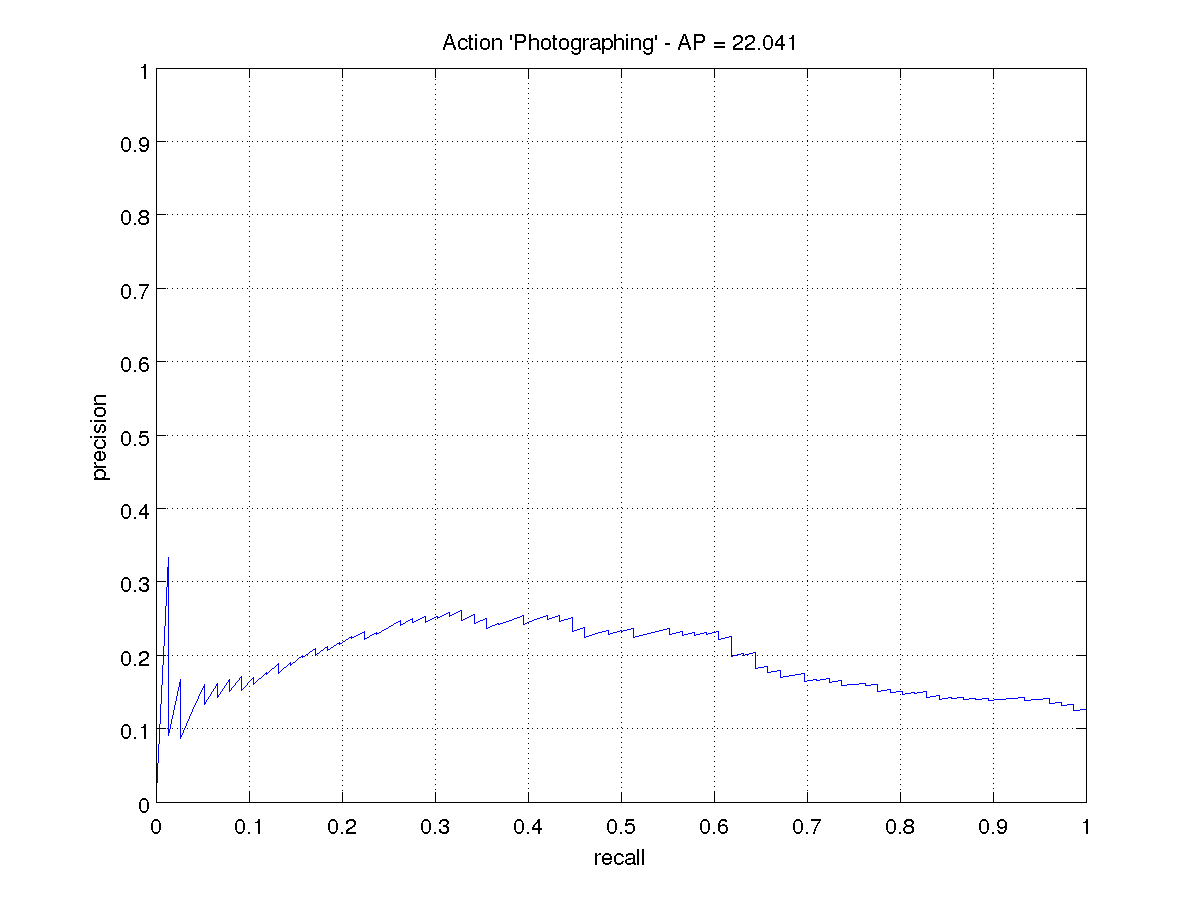
\includegraphics[height=5cm]{img/KNN_BOF_PR_Photographing.png}
\end{minipage}
\begin{minipage}{0.5\linewidth}
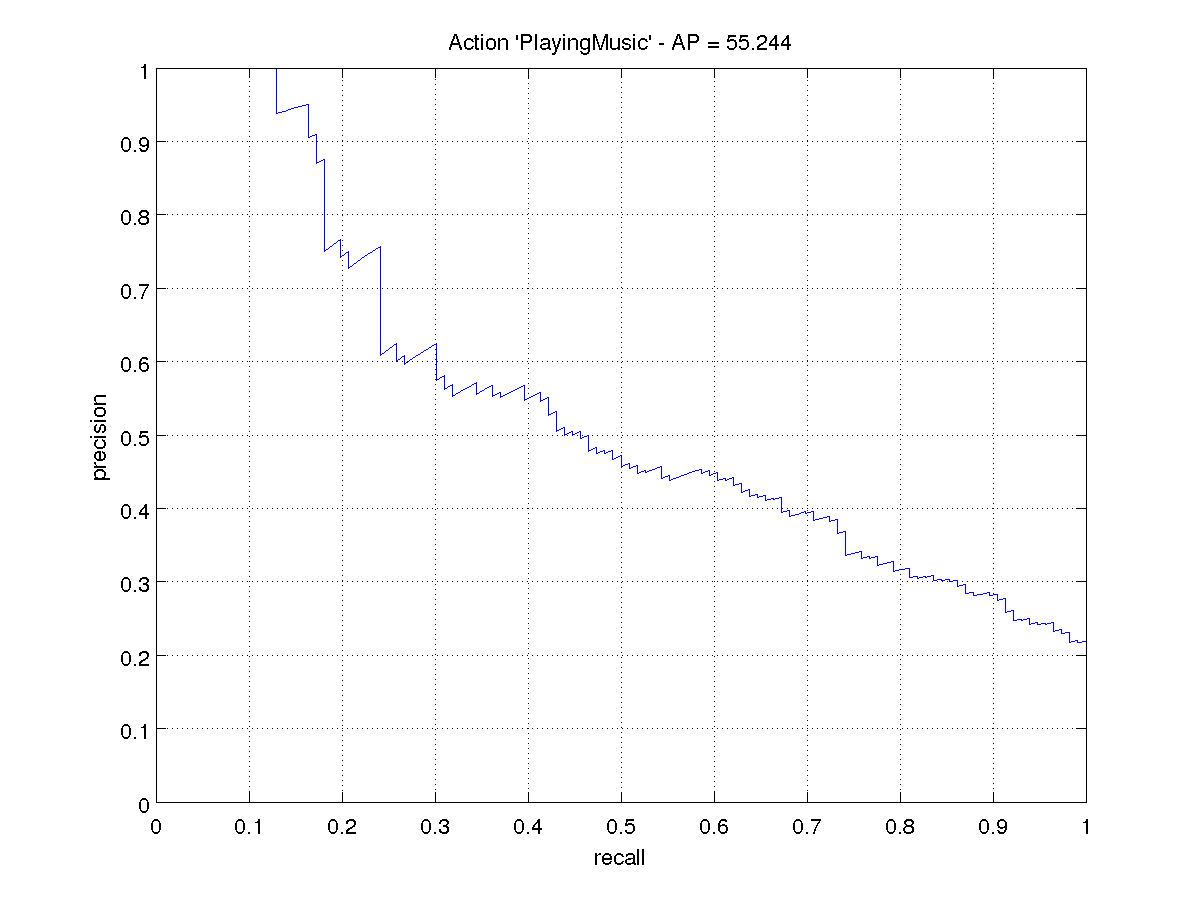
\includegraphics[height=5cm]{img/KNN_BOF_PR_PlayingMusic.png}
\end{minipage}
\begin{minipage}{0.5\linewidth}
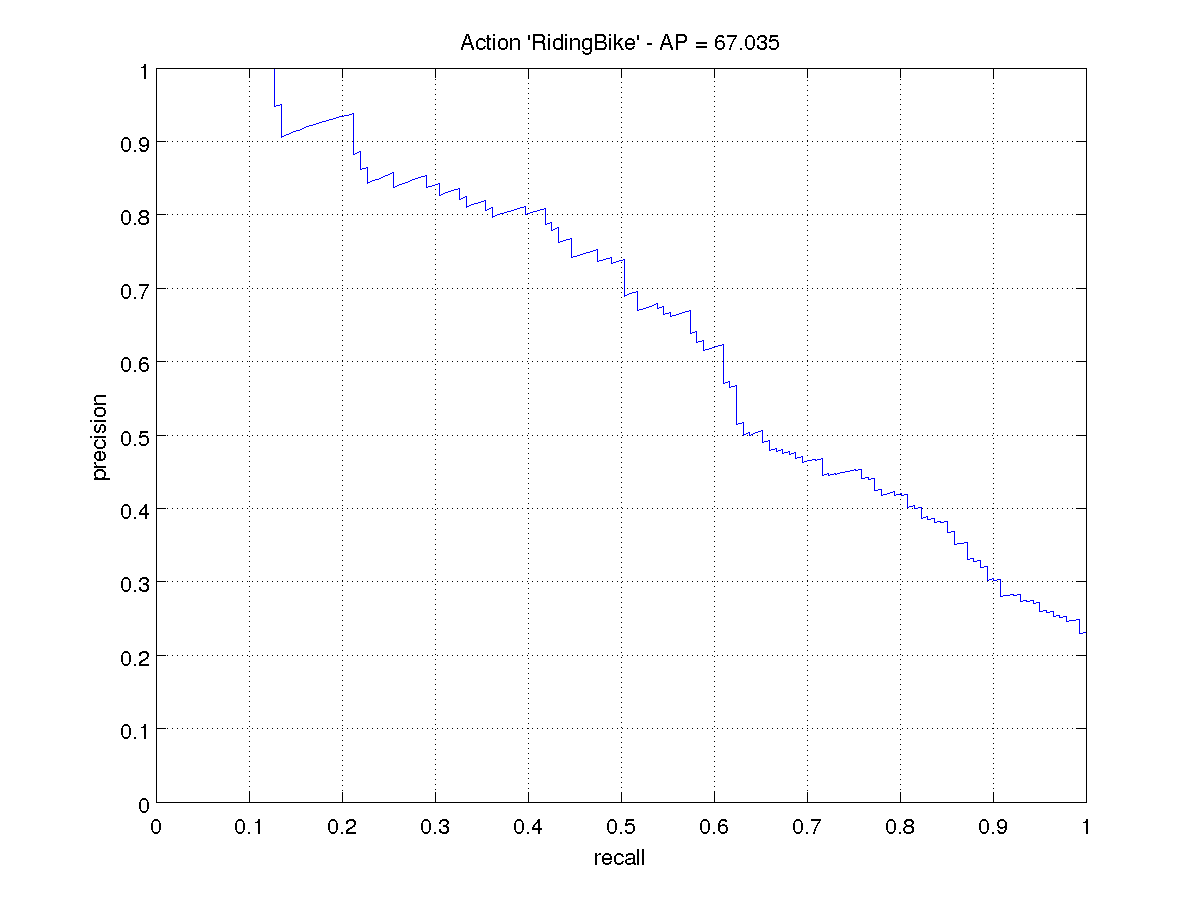
\includegraphics[height=5cm]{img/KNN_BOF_PR_RidingBike.png}
\end{minipage}
\begin{minipage}{0.5\linewidth}
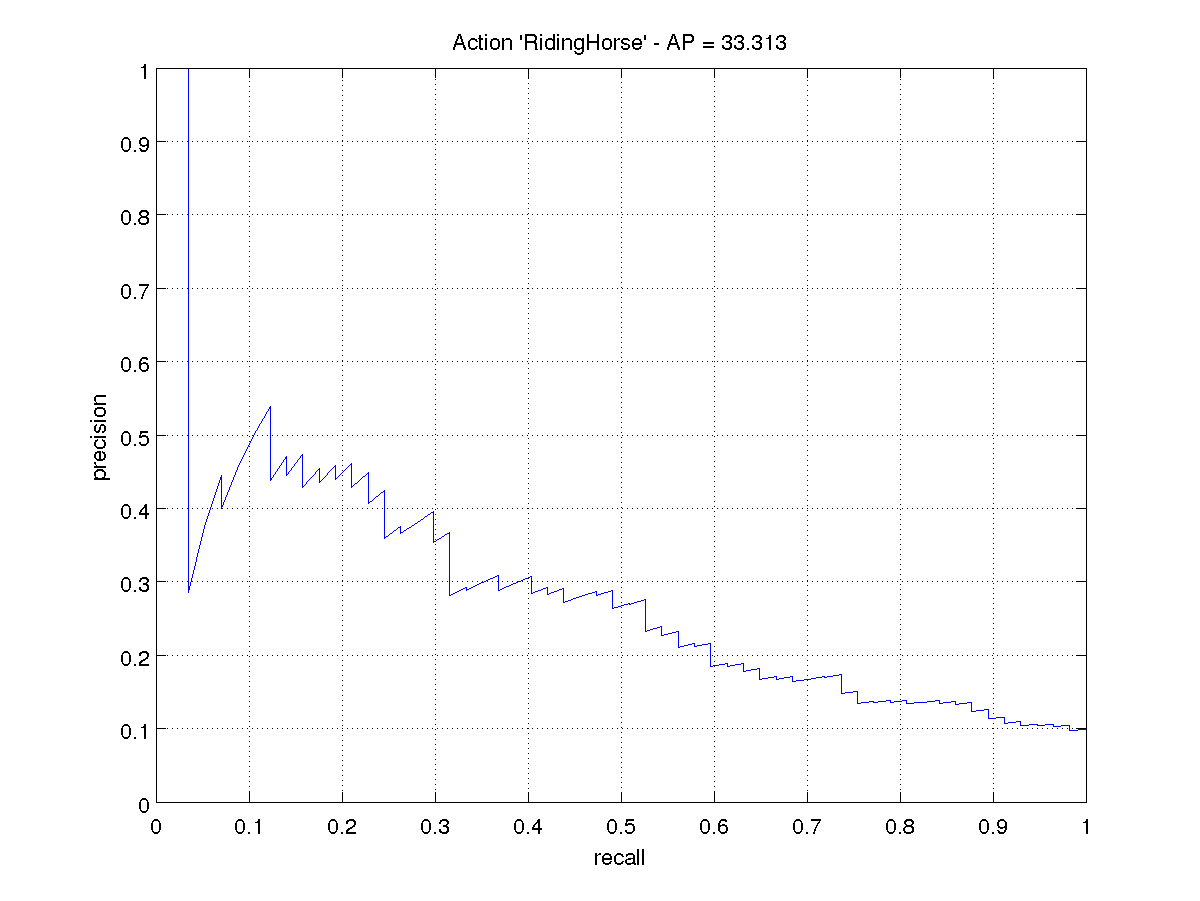
\includegraphics[height=5cm]{img/KNN_BOF_PR_RidingHorse.png}
\end{minipage}
\begin{minipage}{0.5\linewidth}
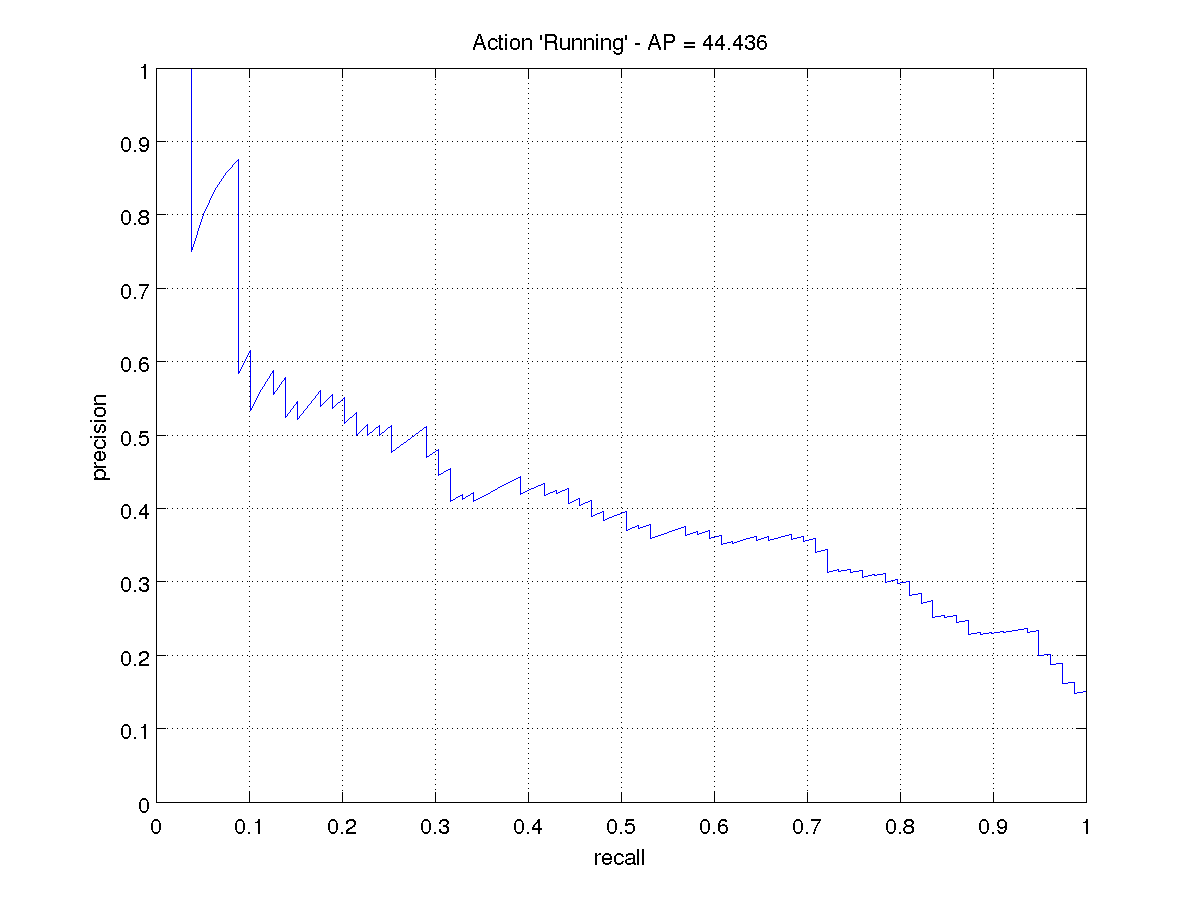
\includegraphics[height=5cm]{img/KNN_BOF_PR_Running.png}
\end{minipage}
\begin{minipage}{0.5\linewidth}
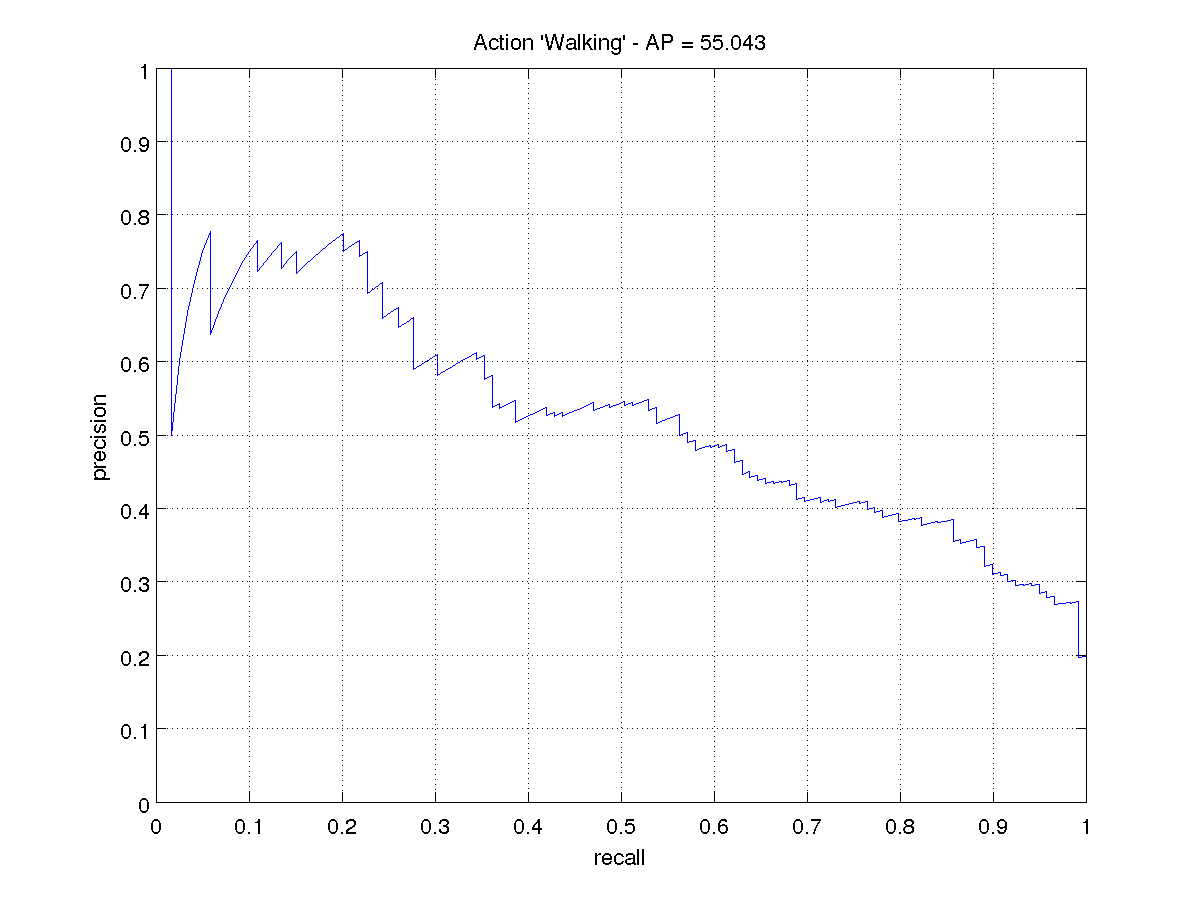
\includegraphics[height=5cm]{img/KNN_BOF_PR_Walking.png}
\end{minipage}
\end{figure}


\newpage
% ===============================================================================%
\section{SVM classifier + Bag-of-features}
%--------------------------------------------------------------------------------%
\subsection{Tested Parameters}

\subsubsection{Detectors}$~$\\
\begin{itemize}
\item MSDENSE: Multi-scale dense features.
\end{itemize}

\subsubsection{Descriptors}$~$\\
\begin{itemize}
\item SIFT(L2): SIFT descriptor normalized with L2 norm.
\item SIFT(L2T): SIFT descriptor normalized with L2 norm and truncation over 0.2.
\end{itemize}

\subsubsection{Dictionnary size}$~$\\
Tested sizes: 256, 512, 1024.

\subsubsection{Histogram normalization}$~$\\
\begin{itemize}
\item NONE: no normalization.
\item L1: normalized with L1 norm.
\item L2: normalized with L2 norm.
\end{itemize}

\subsubsection{Kernels}$~$\\
\begin{itemize}
\item LINEAR: linear SVM.
\item RBF: non linear SVM with RBF kernel.
\item INTER: non linear SVM with histogram intersection kernel.
\item CHI2: non linear SVM with $\chi^2$ kernel.
\end{itemize}

\subsubsection{Classifier}$~$\\
\begin{itemize}
\item 1vs1: One-versus-one classification
\item 1vsA: One-versus-all classification
\end{itemize}

%--------------------------------------------------------------------------------%
\subsection{Results}

\subsubsection{Descriptor}$~$\\

\begin{table}[H]
\centering
\caption{SVM+BOF: Average performances for different descriptors. The mean is computed over all other combinaison of parameters.}
\label{table:SVM_BOF:Descriptor}
\begin{tabular}{|l|c|c|}
\hline
$~~$Descriptor & SIFT(L2) & SIFT(L2T) \\ \hline
$~~$Avg. perf.$~~$ & $~~\mathbf{45.4 \pm 3.6}~~$ & $~~45.1 \pm 3.3~~$ \\ \hline
\end{tabular}
\end{table}

\subsubsection{Dictionnary size}$~$\\

\begin{table}[H]
\centering
\caption{SVM+BOF: Average performances for different dictionnary size. The mean is computed over all other combinaison of parameters.}
\label{table:SVM_BOF:DicSize}
\begin{tabular}{|l|c|c|c|c|}
\hline
$~~$Dic. Size & 256 & 512 & 1024 \\ \hline
$~~$Avg. perf.$~~$ & $~~44.5 \pm 3.5~~$ & $~~45.2 \pm 3.4~~$ & $~~\mathbf{46.2 \pm 3.2}~~$ \\ \hline
\end{tabular}
\end{table}

\subsubsection{Histogram normalization}$~$\\

\begin{table}[H]
\centering
\caption{SVM+BOF: Average performances for different normalization of the signature histogram. The mean is computed over all other combinaison of parameters.}
\label{table:SVM_BOF:Histonorm}
\begin{tabular}{|l|c|c|c|}
\hline
$~~$Histo. Norm & NONE & L1 & L2 \\ \hline
$~~$Avg. perf.$~~$ & $~~44.4 \pm 4.0~~$ & $~~45.3 \pm 3.4~~$ & $~~\mathbf{46.1 \pm 2.7}~~$ \\ \hline
\end{tabular}
\end{table}


\begin{figure}[H]
\centering
\caption{SVM+BOF: Performances for several kernels and strategy across different histogram normalization. The mean is computed over all other combinaison of parameters.}
\label{fig:SVM_BOF:SIZE_K_graph}
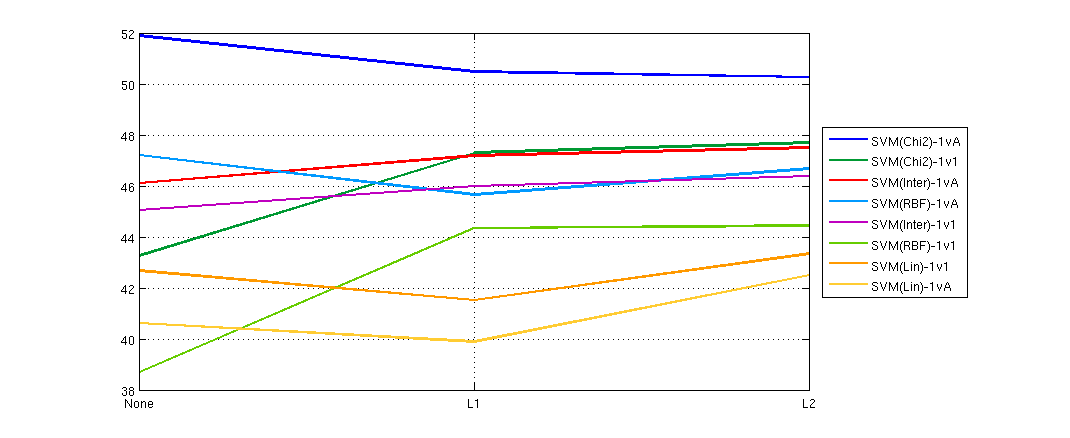
\includegraphics[scale=0.5]{img/SVM_BOF_graph_Norm.png}
\end{figure}

\subsubsection{Kernel}$~$\\

\begin{table}[H]
\centering
\caption{SVM+BOF: Average performances for different kernels. The mean is computed over all other combinaison of parameters.}
\label{table:SVM_BOF:Kernel}
\begin{tabular}{|l|c|c|c|c|}
\hline
$~~$Kernel & LINEAR & RBF & INTER & CHI2\\ \hline
$~~$Avg. perf.$~~$ & $~~41.8 \pm 1.9~~$ & $~~44.5 \pm 3.0~~$ & $~~46.4 \pm 1.3~~$ & $~~\mathbf{48.5 \pm 3.0}~~$\\ \hline
\end{tabular}
\end{table}

\subsubsection{Classifier}$~$\\

\begin{table}[H]
\centering
\caption{SVM+BOF: Average performances for different strategy of classification. The mean is computed over all other combinaison of parameters.}
\label{table:SVM_BOF:Classifier}
\begin{tabular}{|l|c|c|c|}
\hline
$~~$Strategy & 1vs1 & 1vsA \\ \hline
$~~$Avg. perf.$~~$ & $~~44.2 \pm 2.7~~$ & $~~\mathbf{46.3 \pm 3.8}~~$ \\ \hline
\end{tabular}
\end{table}

%--------------------------------------------------------------------------------%
\subsection{Accurracy and Precision-Recall}

Classifier: SVM one VS all (C = 0.03389, J = 1), 5-fold cross-validation\\
Chi2 kernel: exp(-1/655.8768*$Chi2(X,Y)^2$)\\
Signature: Bag of features (K = 512)\\
Histogram normalization: None\\
K-means library: cpp\\
Channels:\\
(DENSE[spacing = 12-14-17-20-24-29-35-42-51-61, library: mylib]) x (SIFT[normalization: L2 (norm = 1, truncation over 0.2), library: colorDescriptor])\\

\begin{table}[H]
\centering
\caption{SVM+BOF: Confusion table. The average accurracy is \textbf{48.8\%}.}
\label{table:SVM_BOF:Accuracy}
\rowcolors[]{1}{white}{gray!10}
\begin{tabular}{|l|c|c|c|c|c|c|c|}
\hline
$Actions $ & $~~$(1)$~~$ & $~~$(2)$~~$ & $~~$(3)$~~$ & $~~$(4)$~~$ & $~~$(5)$~~$ & $~~$(6)$~~$ & $~~$(7)$~~$\\ \hline
(1) Interacting With Computer & \cellcolor{lightgray}\textbf{86.84} & 0.00 & 7.89 & 2.63 & 0.00 & 0.00 & 2.63 \\ \hline
(2) Photographing             & \cellcolor{lightgray}\textbf{32.89} & 6.58 & 17.11 & 1.32 & 3.95 & 10.53 & 27.63 \\ \hline
(3) Playing Music             & 22.41 & 5.17 & \cellcolor{lightgray}\textbf{41.38} & 13.79 & 5.17 & 0.86 & 11.21 \\ \hline
(4) Riding Bike               & 6.38 & 1.42 & 7.09 & \cellcolor{lightgray}\textbf{61.70} & 8.51 & 4.26 & 10.64 \\ \hline
(5) Riding Horse              & 12.28 & 8.77 & 15.79 & 7.02 & \cellcolor{lightgray}\textbf{38.60} & 7.02 & 10.53 \\ \hline
(6) Running                   & 12.66 & 3.80 & 1.27 & 12.66 & 1.27 & \cellcolor{lightgray}\textbf{46.84} & 21.52 \\ \hline
(7) Walking                   & 4.20 & 2.52 & 3.36 & 1.68 & 11.76 & 21.85 & \cellcolor{lightgray}\textbf{54.62} \\ \hline
\end{tabular}
\end{table}


\begin{figure}
\caption{SVM+BOF: Precision-Recall. The average precision is \textbf{51.8\%}.}
\label{fig:SVM_BOF_PR}
\begin{minipage}{0.5\linewidth}
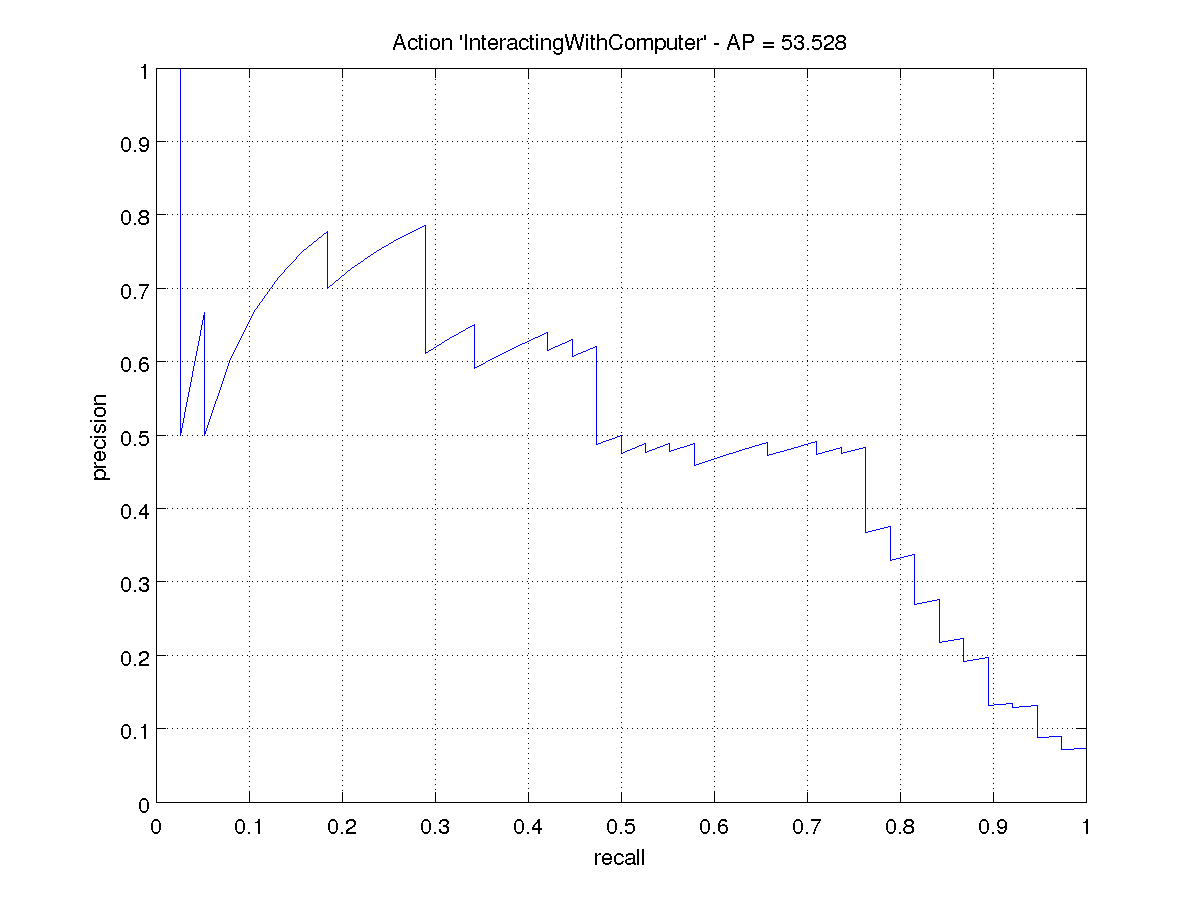
\includegraphics[height=5cm]{img/SVM_BOF_PR_InteractingWithComputer.png}
\end{minipage}
\begin{minipage}{0.5\linewidth}
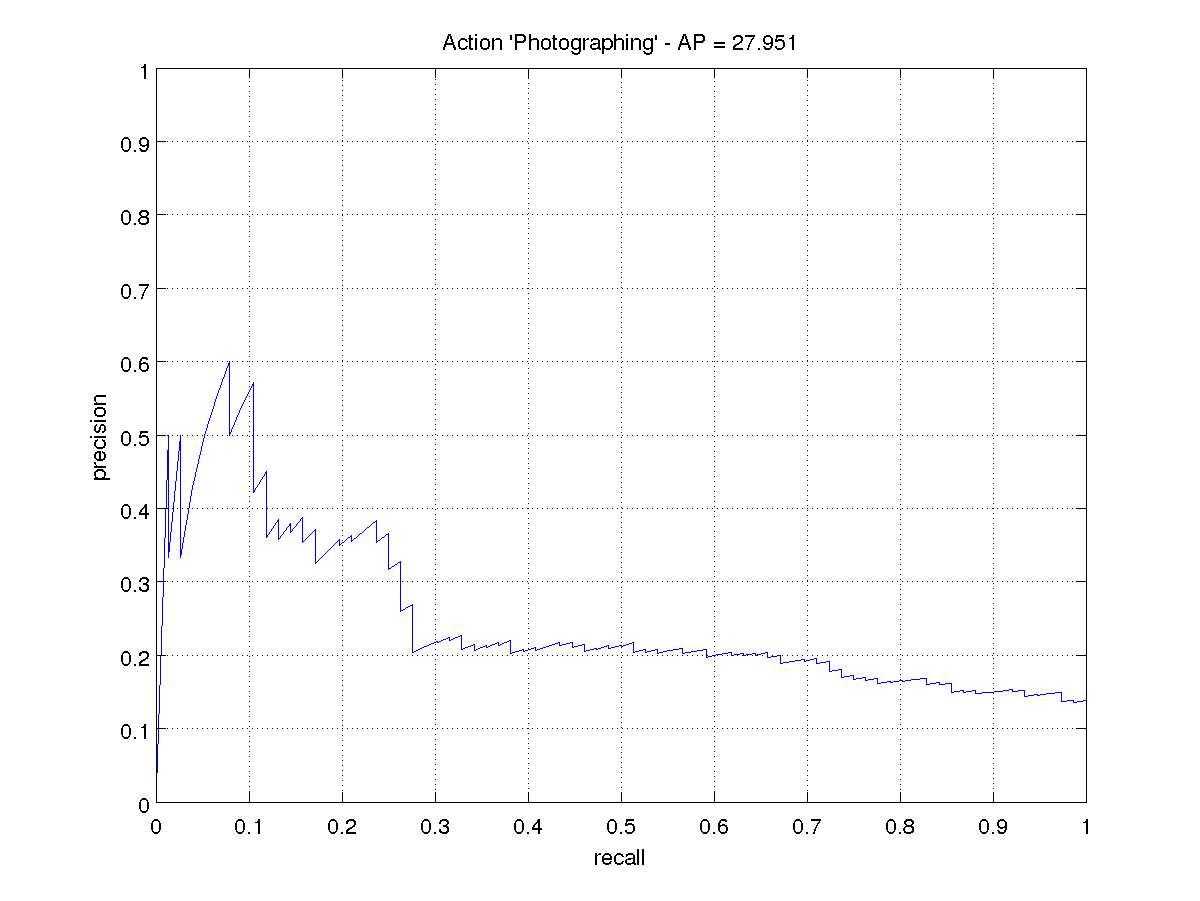
\includegraphics[height=5cm]{img/SVM_BOF_PR_Photographing.png}
\end{minipage}
\begin{minipage}{0.5\linewidth}
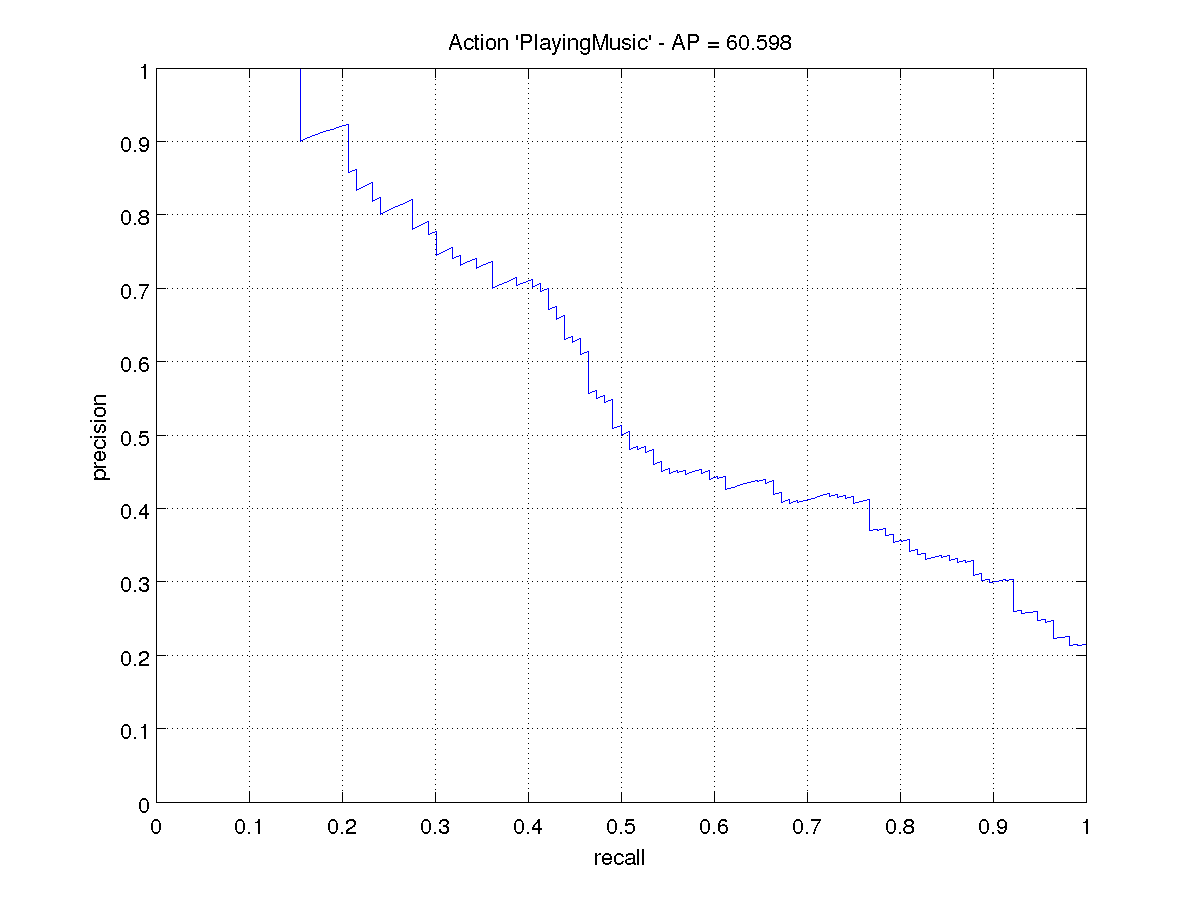
\includegraphics[height=5cm]{img/SVM_BOF_PR_PlayingMusic.png}
\end{minipage}
\begin{minipage}{0.5\linewidth}
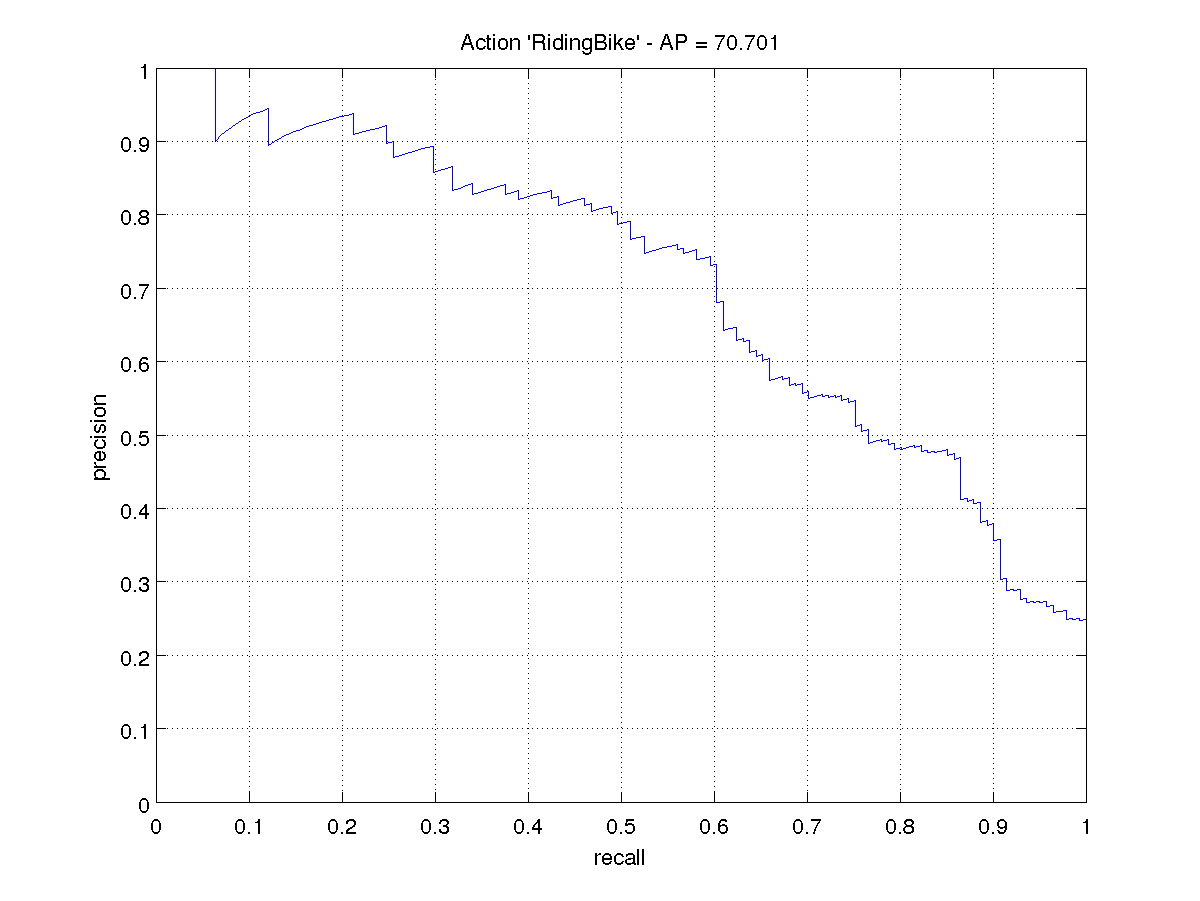
\includegraphics[height=5cm]{img/SVM_BOF_PR_RidingBike.png}
\end{minipage}
\begin{minipage}{0.5\linewidth}
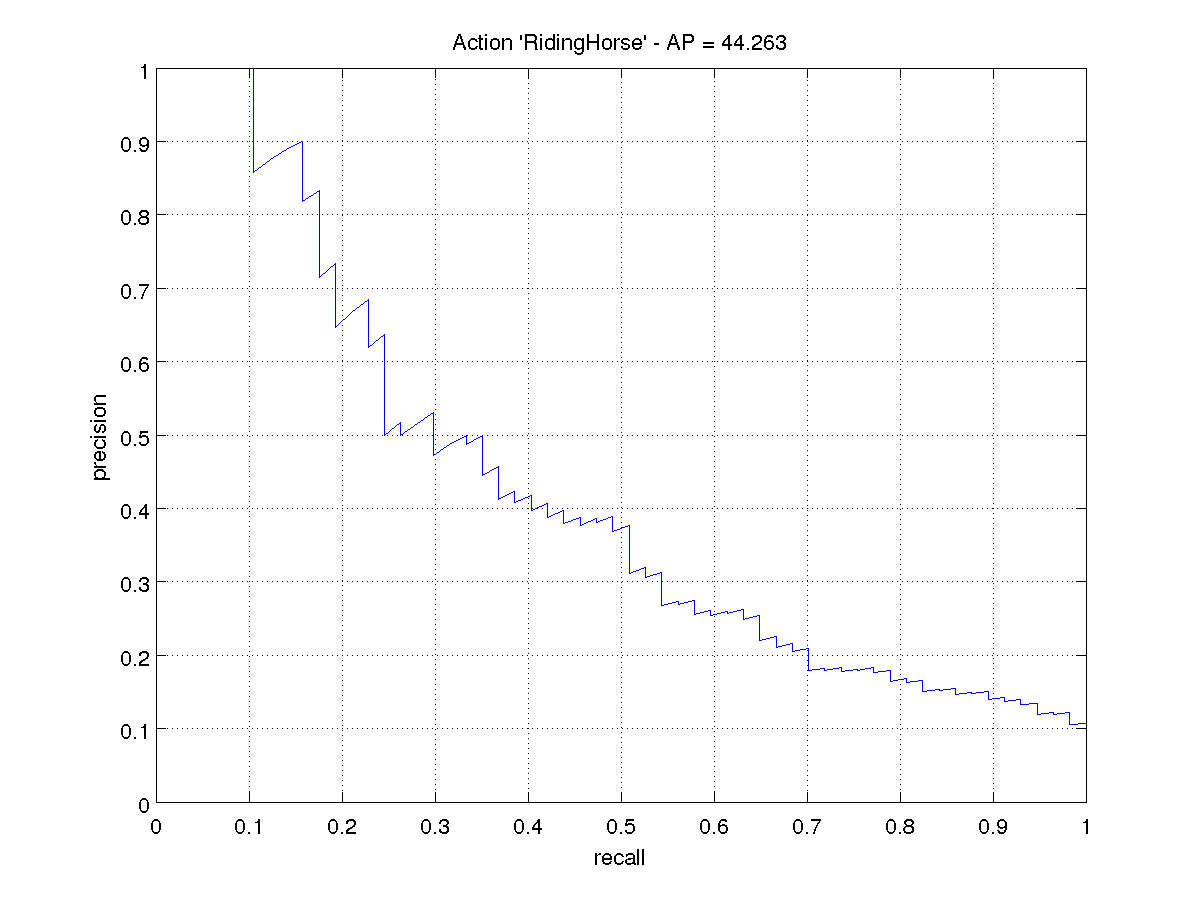
\includegraphics[height=5cm]{img/SVM_BOF_PR_RidingHorse.png}
\end{minipage}
\begin{minipage}{0.5\linewidth}
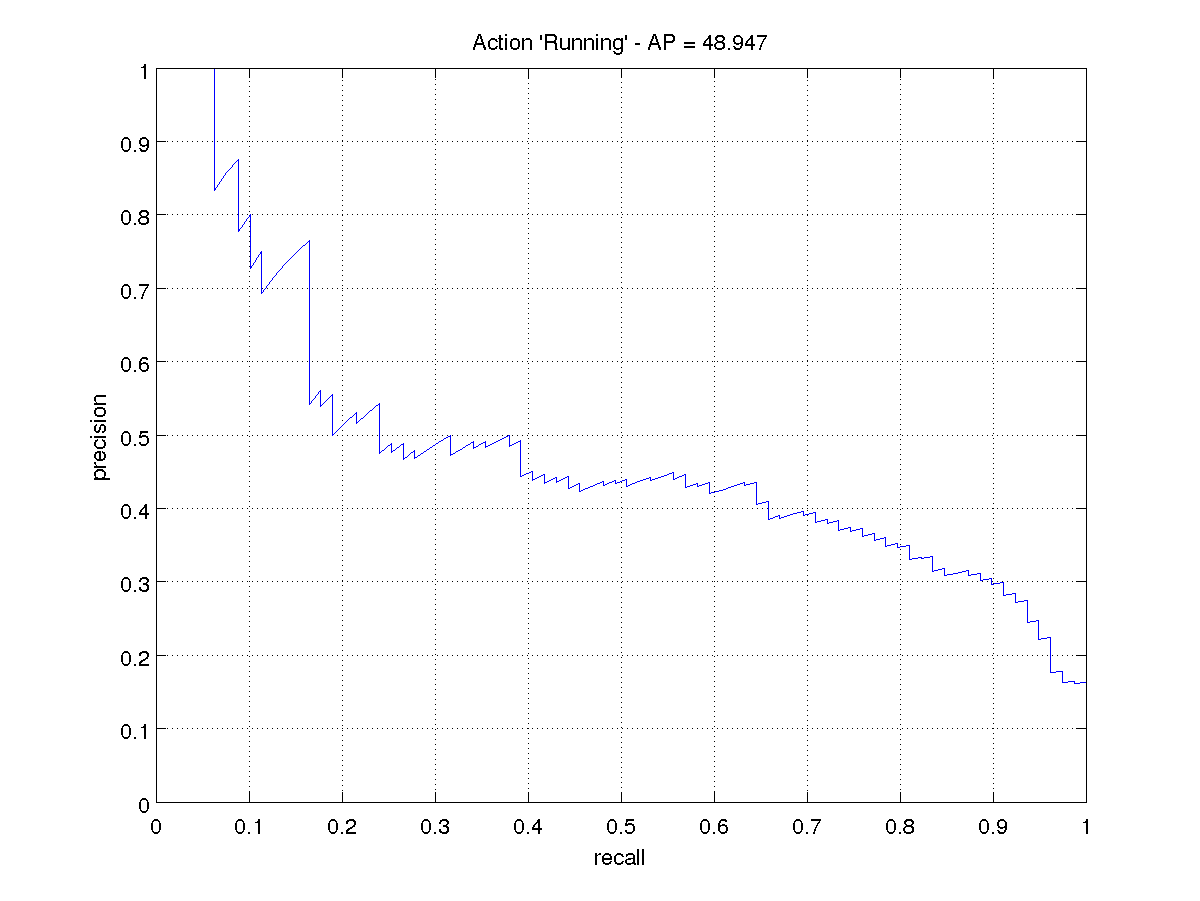
\includegraphics[height=5cm]{img/SVM_BOF_PR_Running.png}
\end{minipage}
\begin{minipage}{0.5\linewidth}
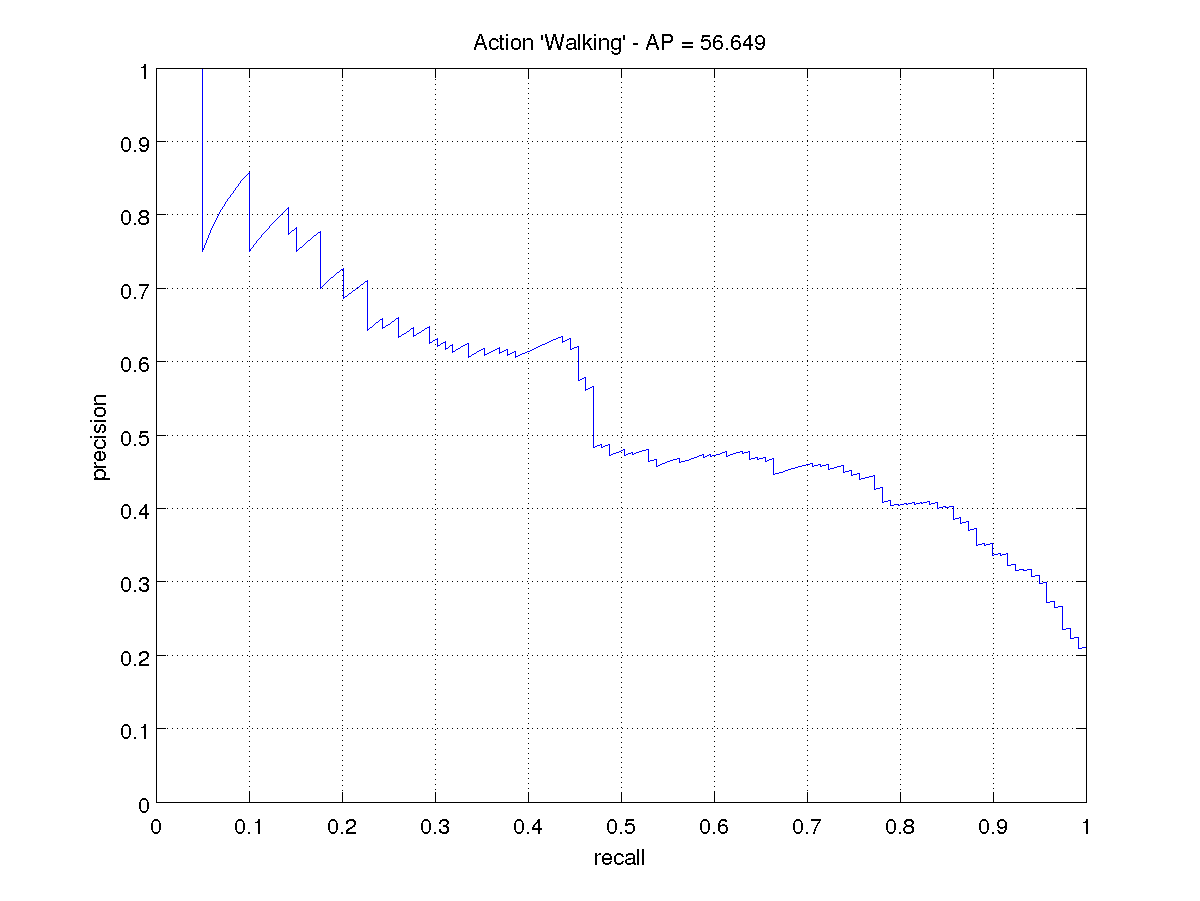
\includegraphics[height=5cm]{img/SVM_BOF_PR_Walking.png}
\end{minipage}
\begin{minipage}{0.5\linewidth}
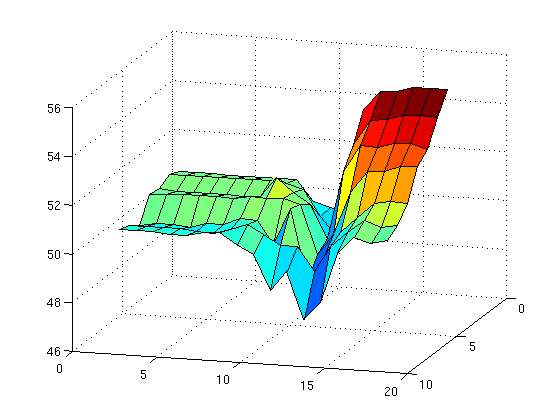
\includegraphics[height=5cm]{img/SVM_BOF_CV.png}
\end{minipage}
\end{figure}

\newpage
% ===============================================================================%
\section{SVM classifier + Spatial Pyramid matching}
%--------------------------------------------------------------------------------%
\subsection{Tested Parameters}

\subsubsection{Detectors}$~$\\
\begin{itemize}
\item MSDENSE: Multi-scale dense features.
\end{itemize}

\subsubsection{Descriptors}$~$\\
\begin{itemize}
\item SIFT(L2): SIFT descriptor normalized with L2 norm.
\item SIFT(L2T): SIFT descriptor normalized with L2 norm and truncation over 0.2.
\end{itemize}

\subsubsection{Dictionnary size}$~$\\
Tested sizes: 256, 512, 1024.

\subsubsection{Number of pyramid levels}$~$\\
Various number of levels were tested: 1, 2 and 3.

\subsubsection{Histogram normalization}$~$\\
\begin{itemize}
\item NONE: no normalization.
\item L1: normalized with L1 norm.
\item L2: normalized with L2 norm.
\end{itemize}

\subsubsection{Classifier}$~$\\
\begin{itemize}
\item 1vs1: One-versus-one classification
\item 1vsA: One-versus-all classification
\end{itemize}

%--------------------------------------------------------------------------------%
\subsection{Results}

\subsubsection{Descriptor}$~$\\

\begin{table}[H]
\centering
\caption{SVM+PYR: Average performances for different descriptors. The mean is computed over all other combinaison of parameters.}
\label{table:SVM_PYR:Descriptor}
\begin{tabular}{|l|c|c|}
\hline
$~~$Descriptor & SIFT(L2) & SIFT(L2T) \\ \hline
$~~$Avg. perf.$~~$ & $~~\mathbf{51.7\pm2.6}~~$ & $~~51.7\pm2.7~~$ \\ \hline
\end{tabular}
\end{table}

\subsubsection{Dictionnary size}$~$\\

\begin{table}[H]
\centering
\caption{SVM+PYR: Average performances for different dictionnary size. The mean is computed over all other combinaison of parameters.}
\label{table:SVM_PYR:DicSize}
\begin{tabular}{|l|c|c|c|c|}
\hline
$~~$Dic. Size & 256 & 512 & 1024 \\ \hline
$~~$Avg. perf.$~~$ & $~~51.3\pm2.6~~$ & $~~\mathbf{52.0\pm2.7}~~$ & $~~51.8\pm2.8~~$ \\ \hline
\end{tabular}
\end{table}

\subsubsection{Histogram normalization}$~$\\

\begin{table}[H]
\centering
\caption{SVM+PYR: Average performances for different normalization of the signature histogram. The mean is computed over all other combinaison of parameters.}
\label{table:SVM_PYR:Histonorm}
\begin{tabular}{|l|c|c|c|}
\hline
$~~$Histo. Norm & NONE & L1 & L2 \\ \hline
$~~$Avg. perf.$~~$ & $~~51.5\pm2.7~~$ & $~~50.8\pm2.6~~$ & $~~\mathbf{52.8\pm2.4}~~$ \\ \hline
\end{tabular}
\end{table}


\subsubsection{Number of pyramid levels}$~$\\

\begin{table}[H]
\centering
\caption{SVM+PYR: Average performances for different number of pyramid levels. The mean is computed over all other combinaison of parameters.}
\label{table:SVM_PYR:Kernel}
\begin{tabular}{|l|c|c|c|}
\hline
$~~$L & 1 & 2 & 3 \\ \hline
$~~$Avg. perf.$~~$ & $~~50.3\pm2.3~~$ & $~~52.4\pm2.5~~$ & $~~\mathbf{52.8\pm2.6}~~$ \\ \hline
\end{tabular}
\end{table}

\subsubsection{Classifier}$~$\\

\begin{table}[H]
\centering
\caption{SVM+PYR: Average performances for different strategy of classification. The mean is computed over all other combinaison of parameters.}
\label{table:SVM_PYR:Classifier}
\begin{tabular}{|l|c|c|c|}
\hline
$~~$Strategy & 1vs1 & 1vsA \\ \hline
$~~$Avg. perf.$~~$ & $~~49.6\pm1.5~~$ & $~~\mathbf{53.8\pm1.8}~~$ \\ \hline
\end{tabular}
\end{table}

%--------------------------------------------------------------------------------%
\subsection{Accurracy and Precision-Recall}

Classifier: SVM one VS all (C = 0.0625, J = 1), 5-fold cross-validation\\
Intersection kernel: sum i(min(Xi,Yi))\\
Signature: Bag of features (K = 512)\\
histogram normalization: L2 (norm = 1)\\
K-means library: cpp\\
Channels:\\
(DENSE[spacing = 12-14-17-20-24-29-35-42-51-61, library: mylib]) x (SIFT[normalization: L2 (norm = 1), library: colorDescriptor])\\

\begin{table}[H]
\centering
\caption{SVM+PYR: Confusion table. The average accurracy is \textbf{55.9\%}.}
\label{table:SVM_PYR:Accuracy}
\rowcolors[]{1}{white}{gray!10}
\begin{tabular}{|l|c|c|c|c|c|c|c|}
\hline
$Actions $ & $~~$(1)$~~$ & $~~$(2)$~~$ & $~~$(3)$~~$ & $~~$(4)$~~$ & $~~$(5)$~~$ & $~~$(6)$~~$ & $~~$(7)$~~$\\ \hline
(1) Interacting With Computer & \cellcolor{lightgray}\textbf{81.58} & 5.26 & 7.89 & 2.63 & 0.00 & 2.63 & 0.00  \\ \hline
(2) Photographing             & 15.79 & 18.42 & 18.42 & 5.26 & 7.89 & 14.47 & \cellcolor{lightgray}\textbf{19.74}  \\ \hline
(3) Playing Music             & 12.93 & 11.21 & \cellcolor{lightgray}\textbf{46.55} & 12.93 & 7.76 & 1.72 & 6.90 \\ \hline
(4) Riding Bike               & 2.13 & 1.42 & 1.42 & \cellcolor{lightgray}\textbf{67.38} & 12.06 & 3.55 & 12.06 \\ \hline
(5) Riding Horse              & 5.26 & 12.28 & 7.02 & 10.53 & \cellcolor{lightgray}\textbf{50.88} & 5.26 & 8.77  \\ \hline
(6) Running                   & 6.33 & 3.80 & 1.27 & 10.13 & 0.00 & \cellcolor{lightgray}\textbf{62.03} & 16.46 \\ \hline
(7) Walking                   & 1.68 & 5.88 & 1.68 & 2.52 & 5.04 & 18.49 & \cellcolor{lightgray}\textbf{64.71} \\ \hline
\end{tabular}
\end{table}

\begin{figure}
\caption{SVM+PYR: Precision-Recall. The average precision is \textbf{56.9\%}.}
\label{fig:SVM_PYR_PR}
\begin{minipage}{0.5\linewidth}
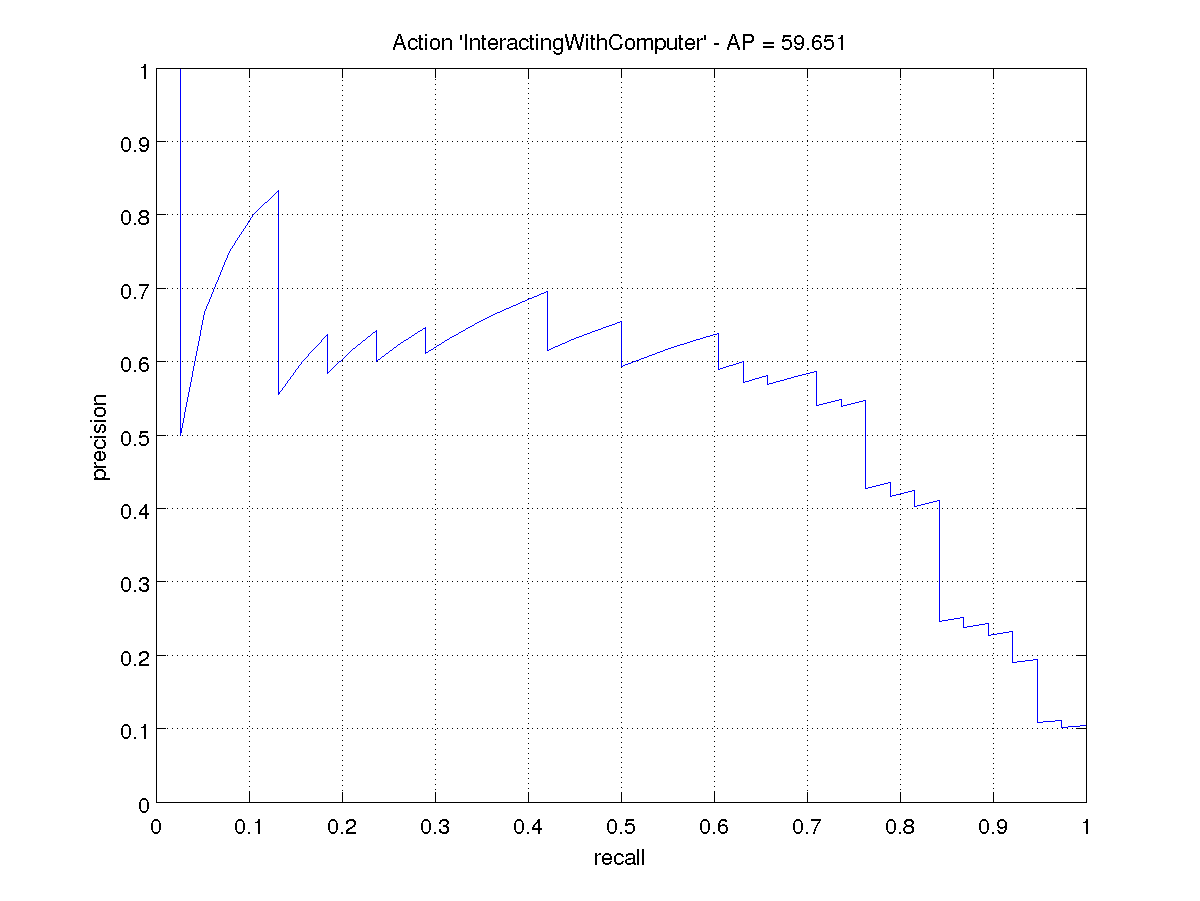
\includegraphics[height=5cm]{img/SVM_PYR_PR_InteractingWithComputer.png}
\end{minipage}
\begin{minipage}{0.5\linewidth}
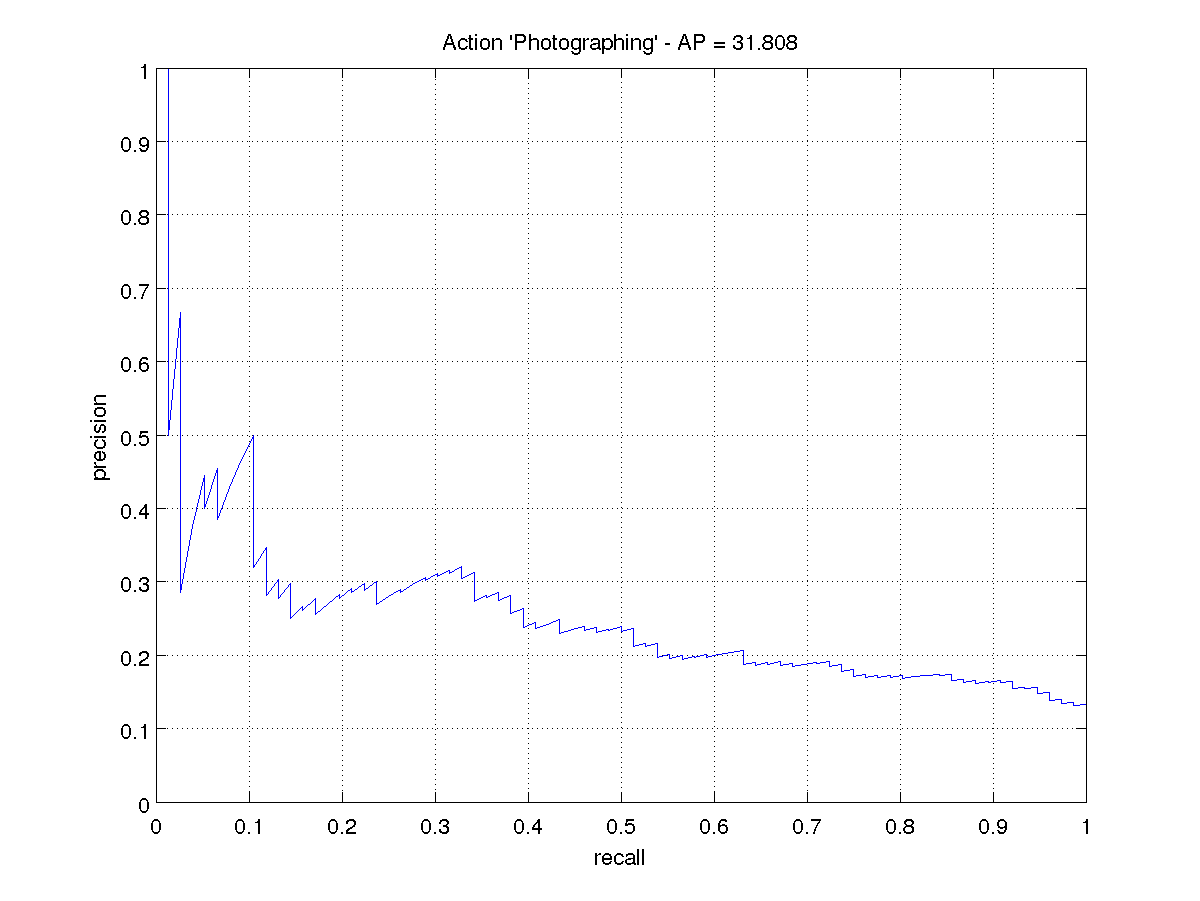
\includegraphics[height=5cm]{img/SVM_PYR_PR_Photographing.png}
\end{minipage}
\begin{minipage}{0.5\linewidth}
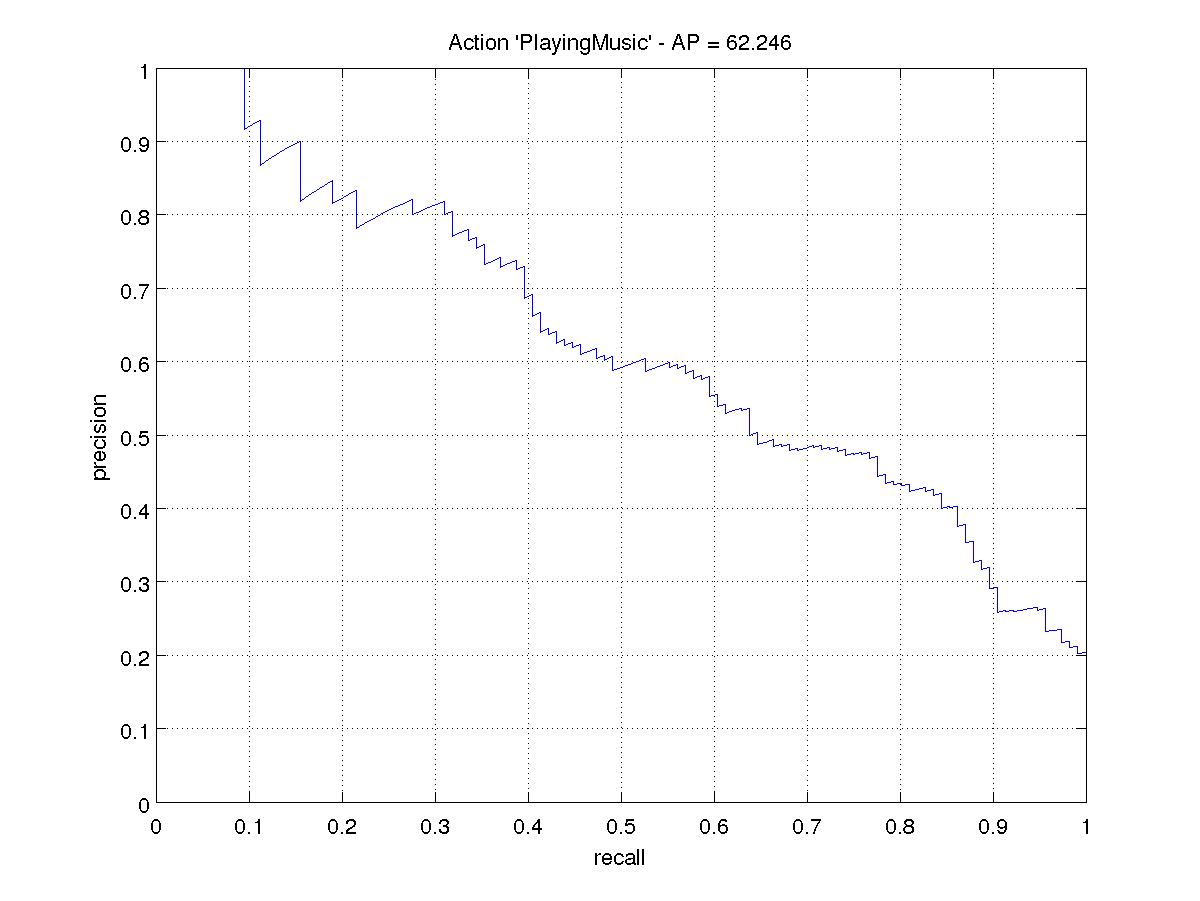
\includegraphics[height=5cm]{img/SVM_PYR_PR_PlayingMusic.png}
\end{minipage}
\begin{minipage}{0.5\linewidth}
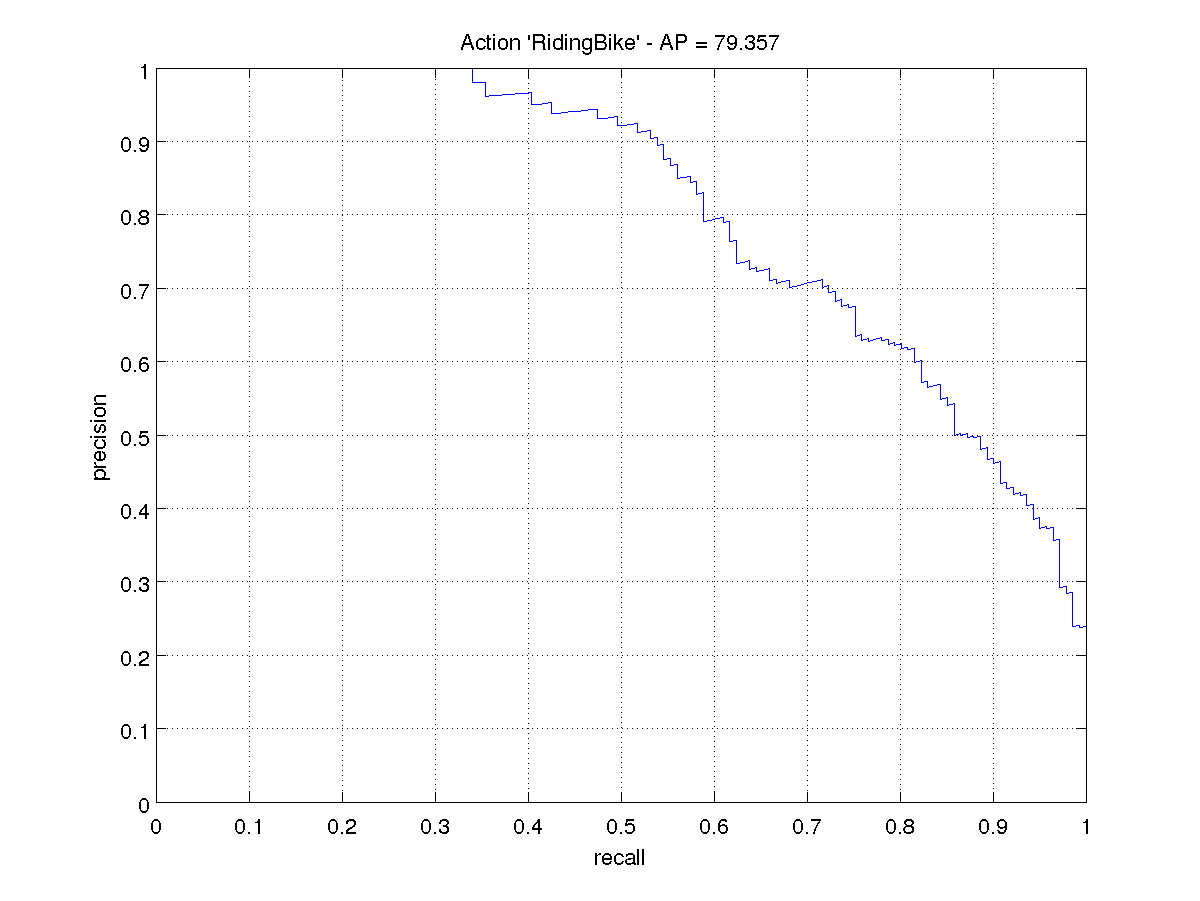
\includegraphics[height=5cm]{img/SVM_PYR_PR_RidingBike.png}
\end{minipage}
\begin{minipage}{0.5\linewidth}
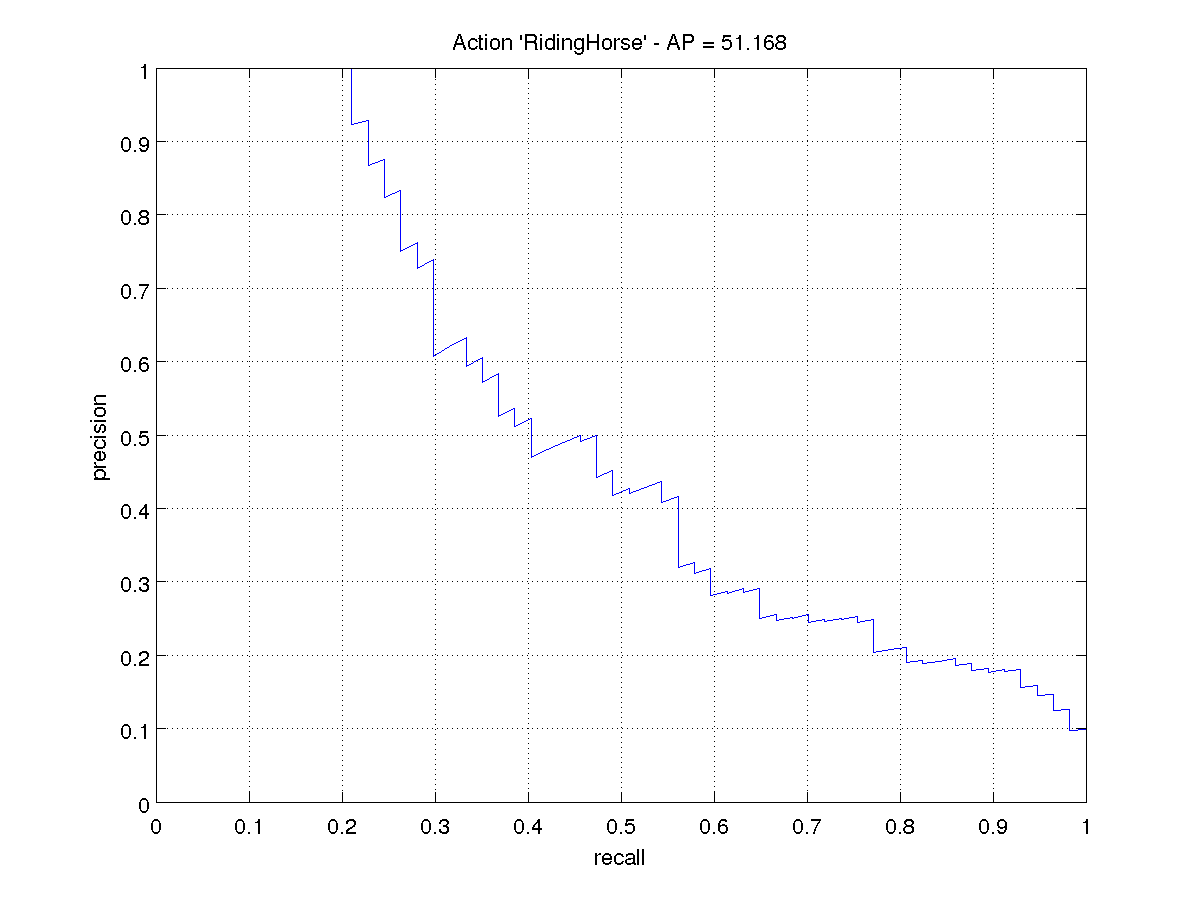
\includegraphics[height=5cm]{img/SVM_PYR_PR_RidingHorse.png}
\end{minipage}
\begin{minipage}{0.5\linewidth}
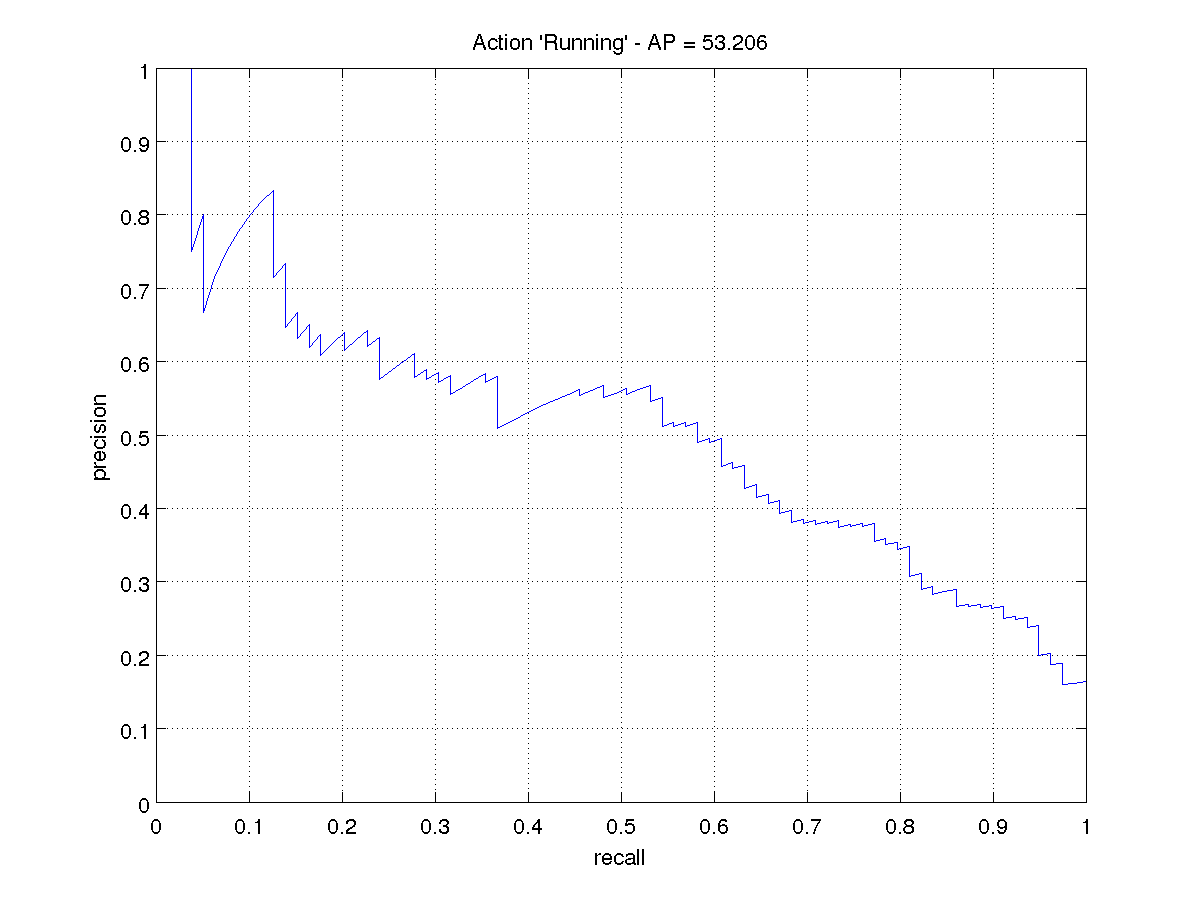
\includegraphics[height=5cm]{img/SVM_PYR_PR_Running.png}
\end{minipage}
\begin{minipage}{0.5\linewidth}
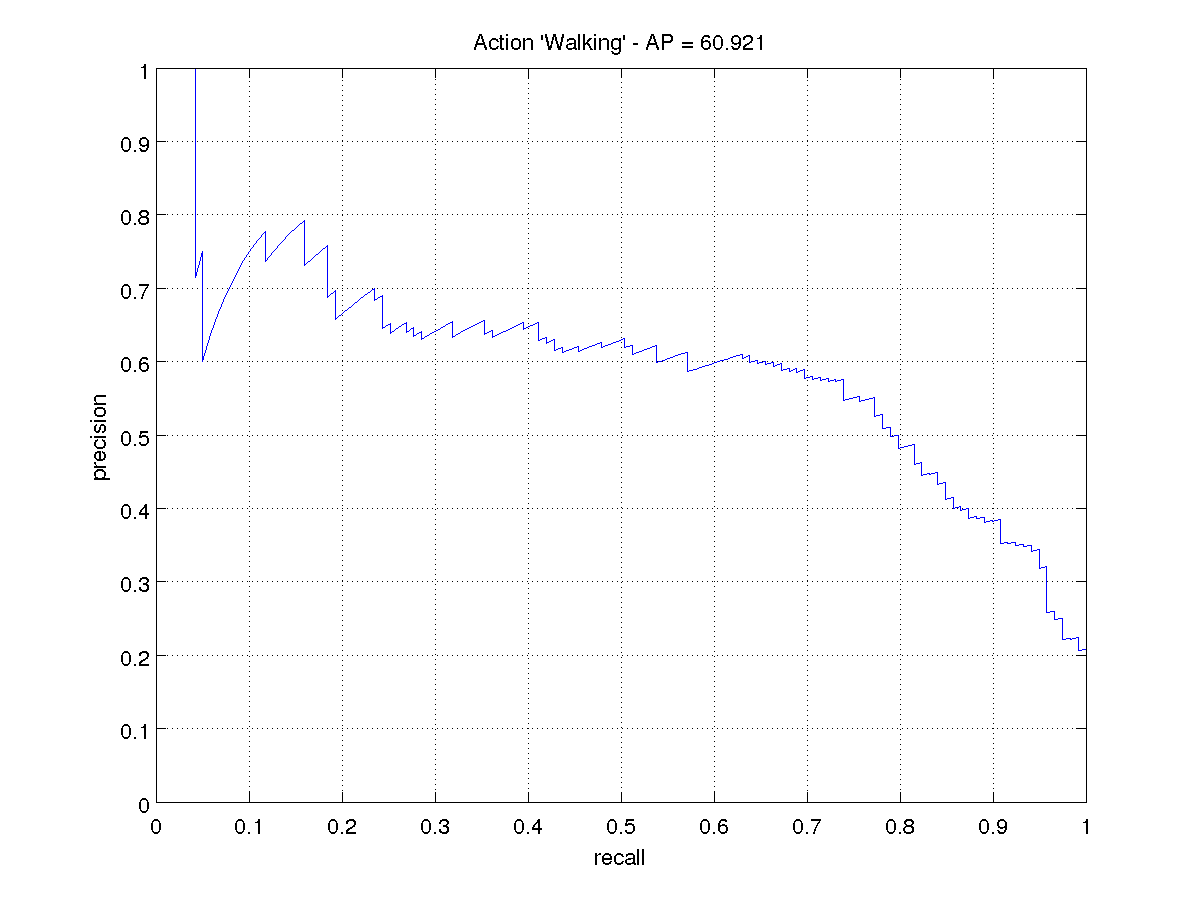
\includegraphics[height=5cm]{img/SVM_PYR_PR_Walking.png}
\end{minipage}
\begin{minipage}{0.5\linewidth}
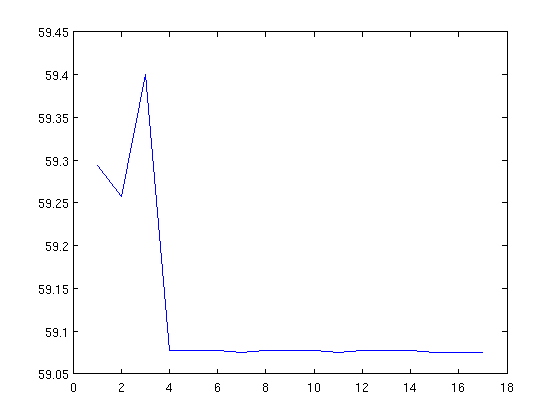
\includegraphics[height=5cm]{img/SVM_PYR_CV.png}
\end{minipage}
\end{figure}


\newpage
% ===============================================================================%
\section{LSVM}
%--------------------------------------------------------------------------------%

\subsection{One component}

Precision: 43.24\%

\begin{table}[H]
\centering
\caption{Confusion table for LSVM with one component. The average accurracy is \textbf{45.55\%}.}
\label{table:LSVM1:Accuracy}
\rowcolors[]{1}{white}{gray!10}
\begin{tabular}{|l|c|c|c|c|c|c|c|}
\hline
$Actions $ & $~~$(1)$~~$ & $~~$(2)$~~$ & $~~$(3)$~~$ & $~~$(4)$~~$ & $~~$(5)$~~$ & $~~$(6)$~~$ & $~~$(7)$~~$ \\ \hline
(1) Interacting With Computer & \cellcolor{lightgray}\textbf{60.53} & 0.00 & 2.63 & 7.89 & 2.63 & 15.79 & 10.53 \\ \hline
(2) Photographing             & 10.53 & 0.00 & 1.32 & 15.79 & \cellcolor{lightgray}\textbf{30.26} & 19.74 & 22.37 \\ \hline
(3) Playing Music             & 16.24 & 0.00 & 2.56 & 24.79 & \cellcolor{lightgray}\textbf{37.61} & 9.40 & 9.40 \\ \hline
(4) Riding Bike               & 0.71 & 0.00 & 1.42 & \cellcolor{lightgray}\textbf{64.54} & 14.89 & 9.22 & 9.22 \\ \hline
(5) Riding Horse              & 0.00 & 0.00 & 0.00 & 16.07 & \cellcolor{lightgray}\textbf{60.71} & 8.93 & 14.29 \\ \hline
(6) Running                   & 2.53 & 0.00 & 0.00 & 10.00 & 3.75 & \cellcolor{lightgray}\textbf{73.15} & 10.00 \\ \hline
(7) Walking                   & 0.85 & 0.00 & 0.00 & 11.02 & 10.17 & 21.19 & \cellcolor{lightgray}\textbf{56.78} \\ \hline
\end{tabular}
\end{table}



\subsection{Two components}

Precision: 43.70\%

\begin{table}[H]
\centering
\caption{Confusion table for LSVM with two components. The average accurracy is \textbf{46.18\%}.}
\label{table:LSVM2:Accuracy}
\rowcolors[]{1}{white}{gray!10}
\begin{tabular}{|l|c|c|c|c|c|c|c|}
\hline
$Actions $ & $~~$(1)$~~$ & $~~$(2)$~~$ & $~~$(3)$~~$ & $~~$(4)$~~$ & $~~$(5)$~~$ & $~~$(6)$~~$ & $~~$(7)$~~$ \\ \hline
(1) Interacting With Computer & \cellcolor{lightgray}\textbf{34.21} & 18.42 & 34.21 & 5.26 & 2.63 & 0.00 & 5.26 \\ \hline
(2) Photographing             & 3.95 & \cellcolor{lightgray}\textbf{34.21} & 25.00 & 10.53 & 13.16 & 3.95 & 9.21 \\ \hline
(3) Playing Music             & 13.68 & 11.11 & \cellcolor{lightgray}\textbf{52.99} & 9.40 & 7.69 & 1.71 & 3.42 \\ \hline
(4) Riding Bike               & 2.84 & 9.22 & 14.18 & \cellcolor{lightgray}\textbf{59.57} & 7.09 & 2.84 & 4.26 \\ \hline
(5) Riding Horse              & 0.00 & 7.14 & 23.21 & 10.71 & \cellcolor{lightgray}\textbf{48.21} & 3.57 & 7.14 \\ \hline
(6) Running                   & 2.50 & 1.25 & 15.00 & 17.50 & 3.75 & \cellcolor{lightgray}\textbf{50.00} & 10.00 \\ \hline
(7) Walking                   & 1.68 & 6.78 & 16.10 & 5.93 & 8.47 & 16.95 & \cellcolor{lightgray}\textbf{44.07} \\ \hline

\end{tabular}
\end{table}

\begin{figure}
\caption{LSVM: Precision-Recall. The average precision is \textbf{43.70\%}.}
\label{fig:LSVM_PR}
\begin{minipage}{0.5\linewidth}
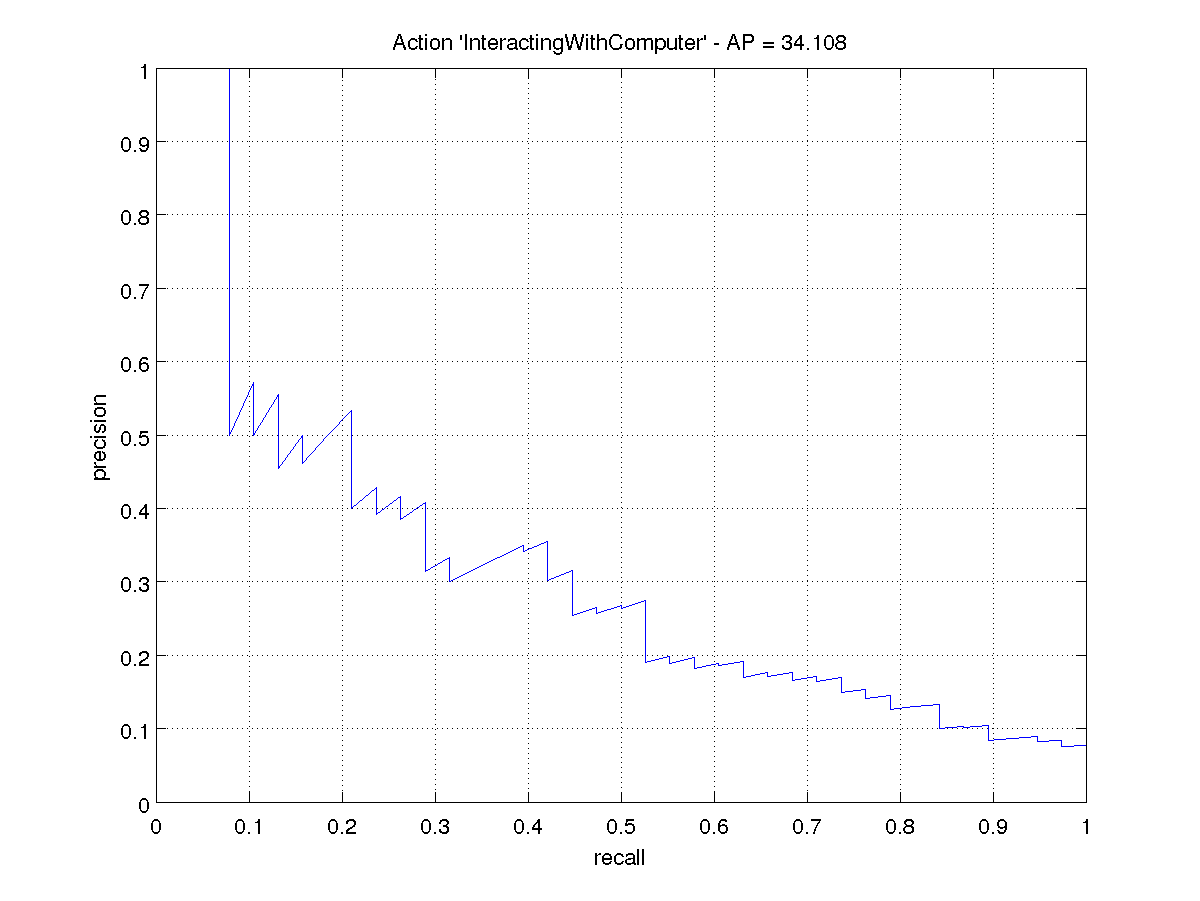
\includegraphics[height=5cm]{img/LSVM_PR_InteractingWithComputer.png}
\end{minipage}
\begin{minipage}{0.5\linewidth}
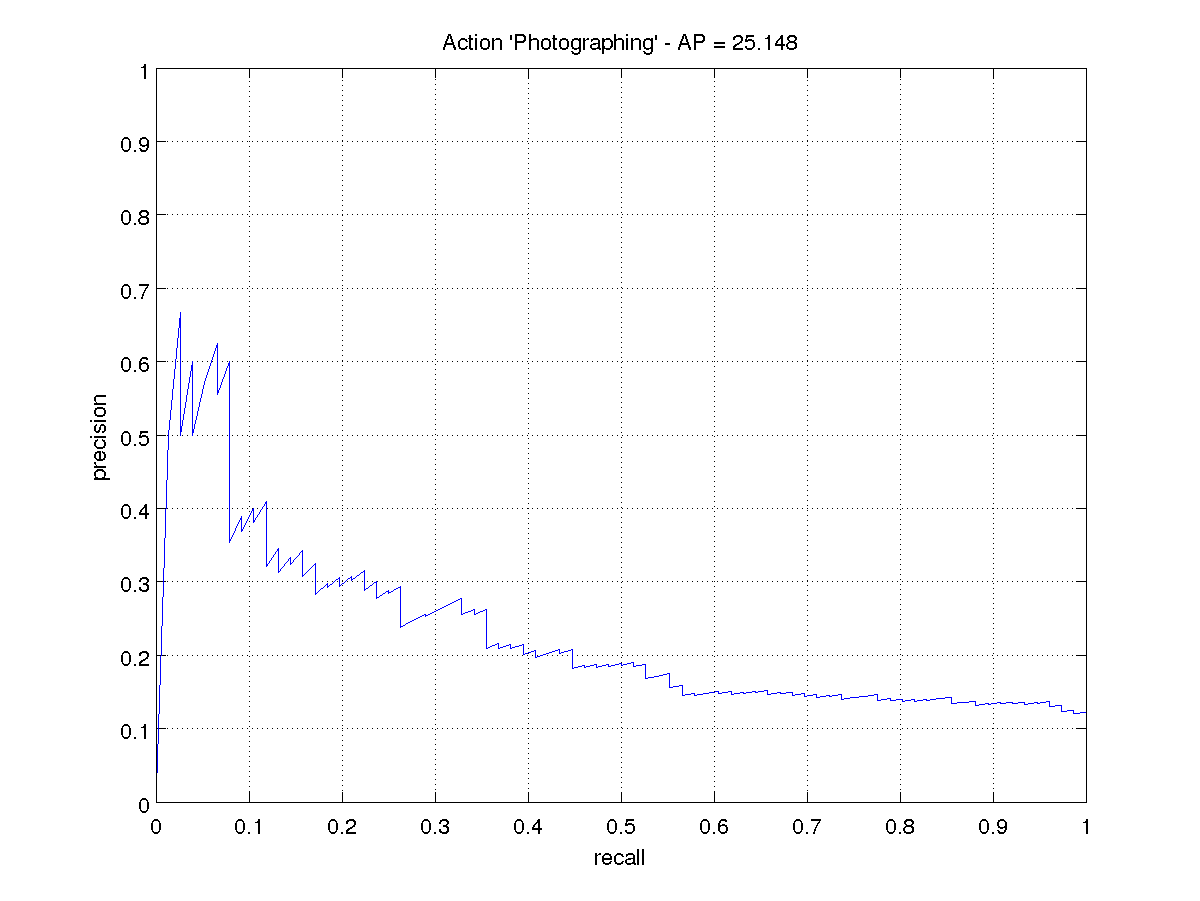
\includegraphics[height=5cm]{img/LSVM_PR_Photographing.png}
\end{minipage}
\begin{minipage}{0.5\linewidth}
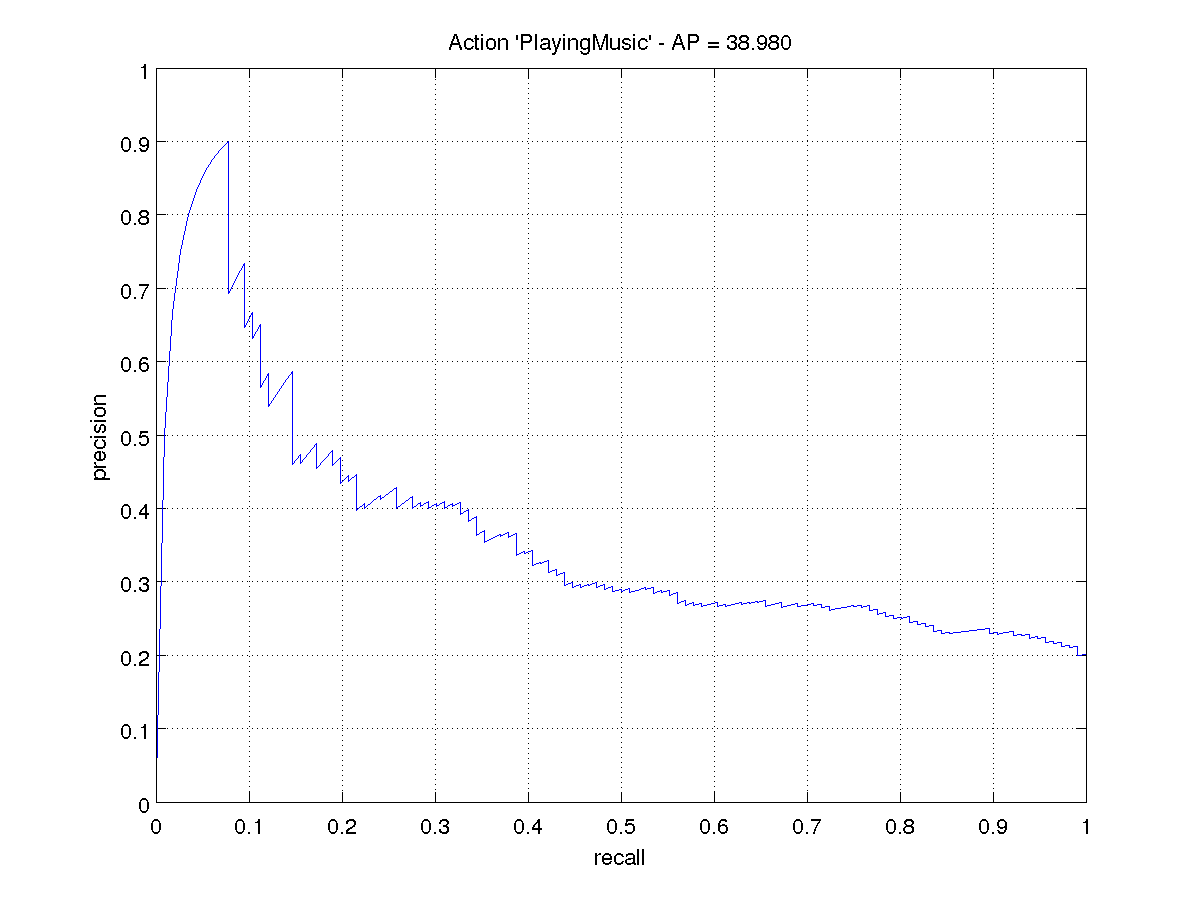
\includegraphics[height=5cm]{img/LSVM_PR_PlayingMusic.png}
\end{minipage}
\begin{minipage}{0.5\linewidth}
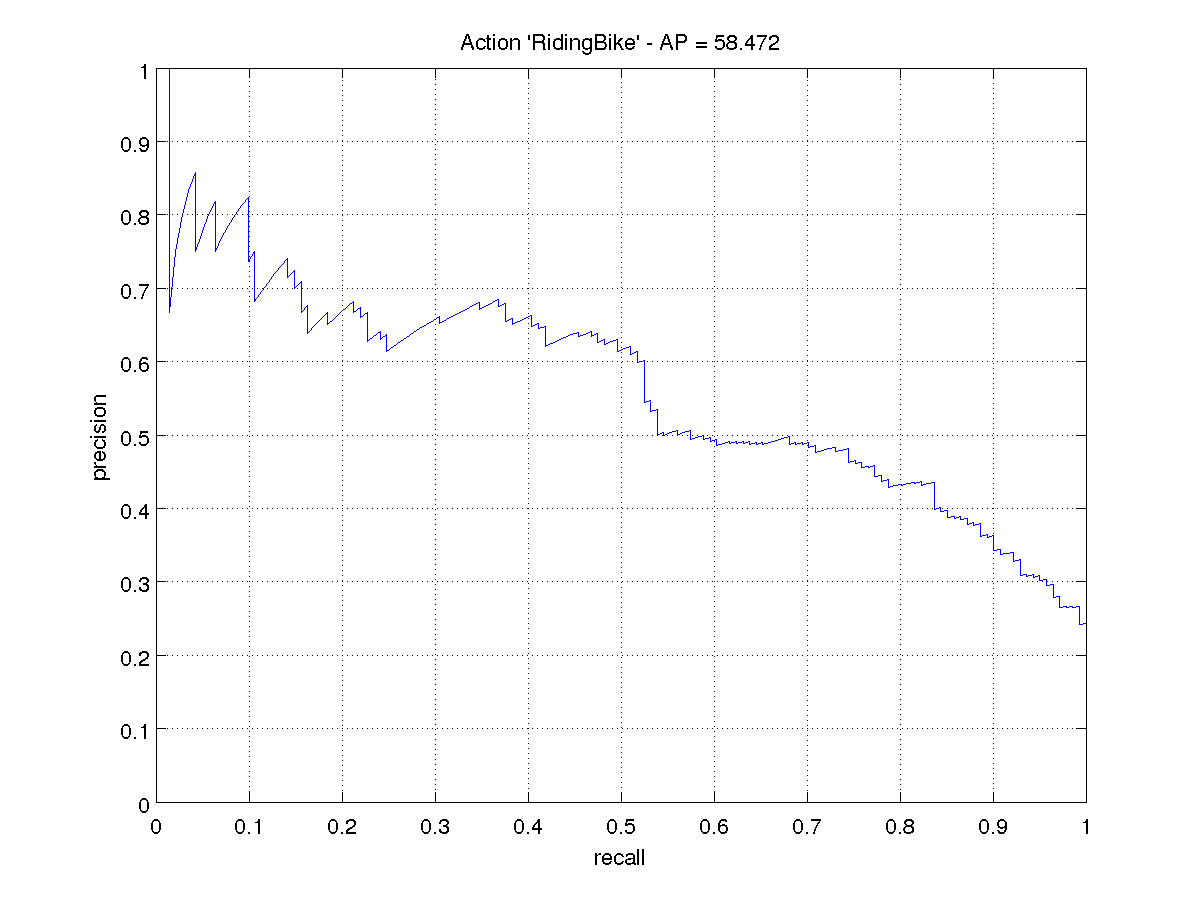
\includegraphics[height=5cm]{img/LSVM_PR_RidingBike.png}
\end{minipage}
\begin{minipage}{0.5\linewidth}
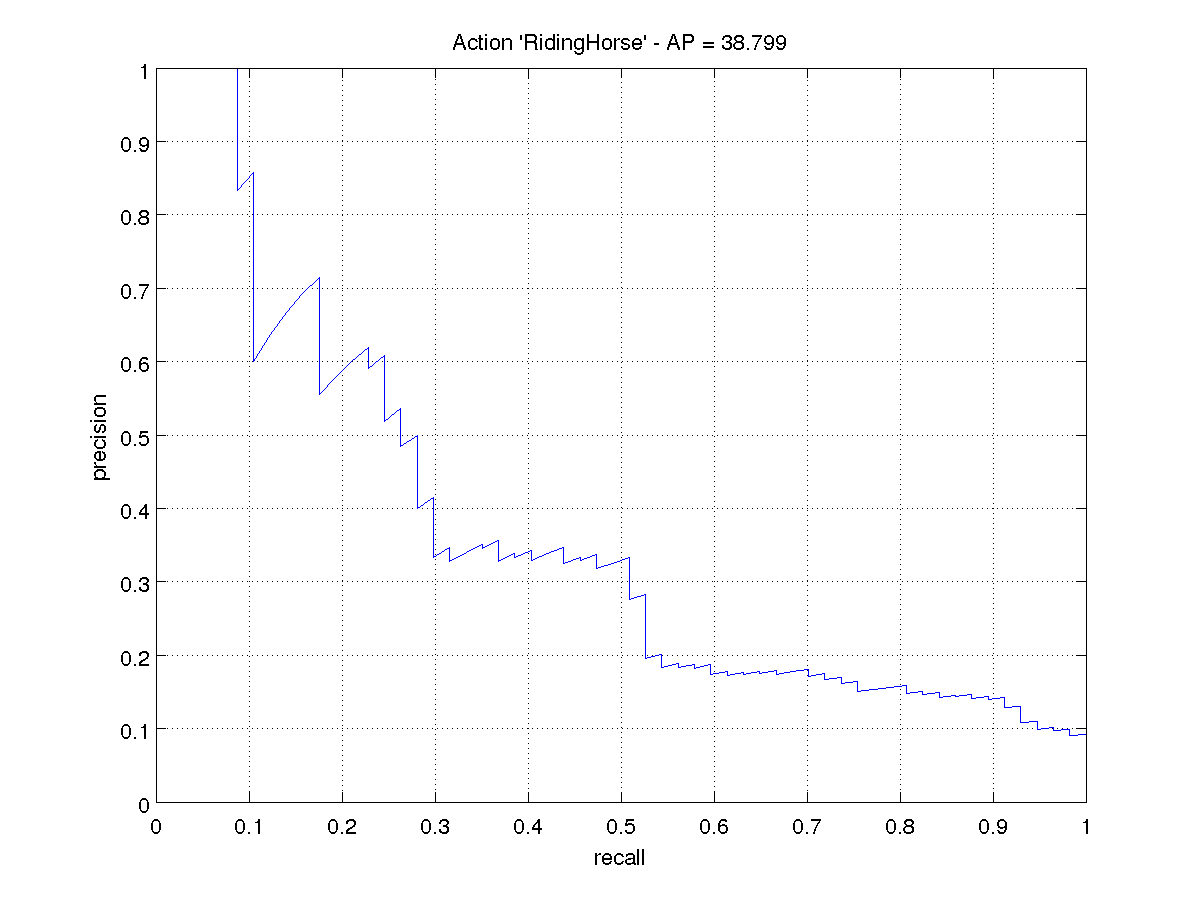
\includegraphics[height=5cm]{img/LSVM_PR_RidingHorse.png}
\end{minipage}
\begin{minipage}{0.5\linewidth}
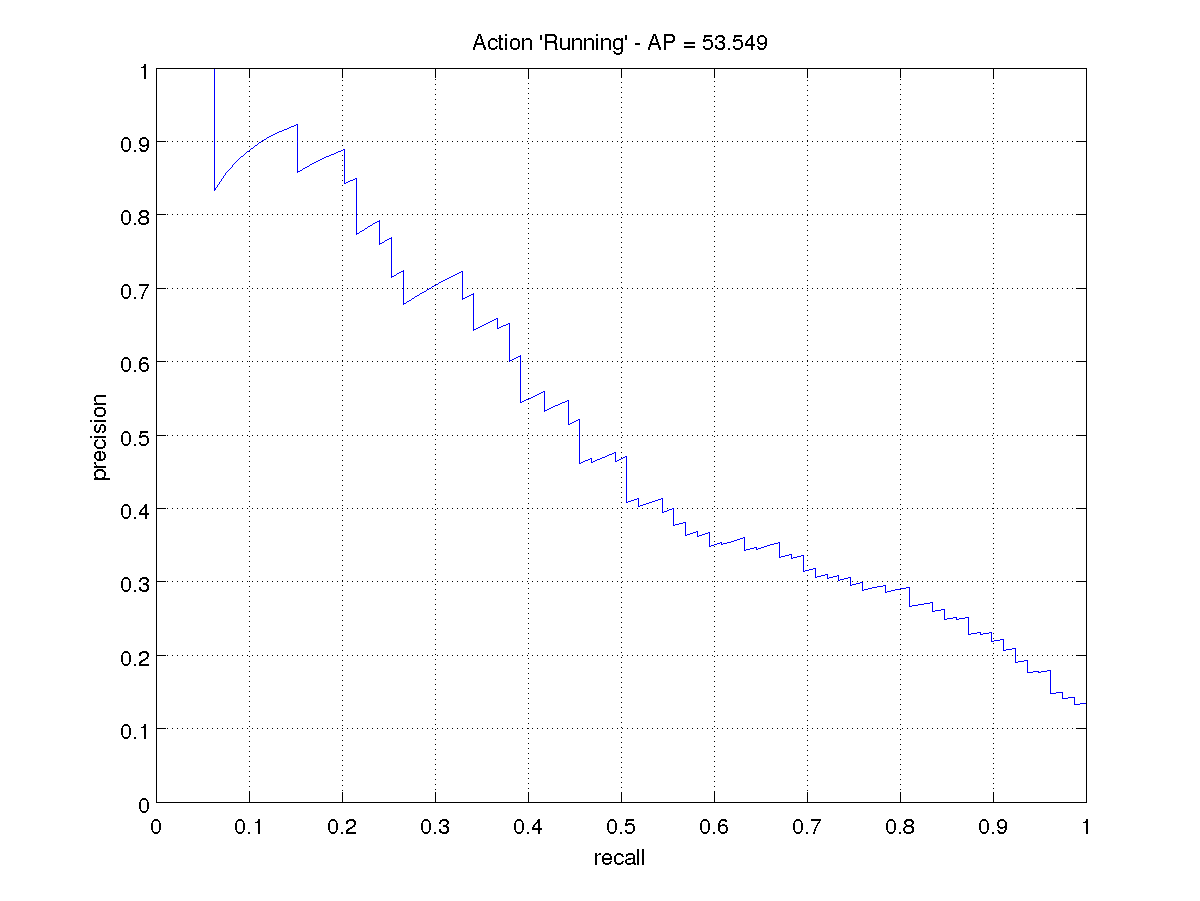
\includegraphics[height=5cm]{img/LSVM_PR_Running.png}
\end{minipage}
\begin{minipage}{0.5\linewidth}
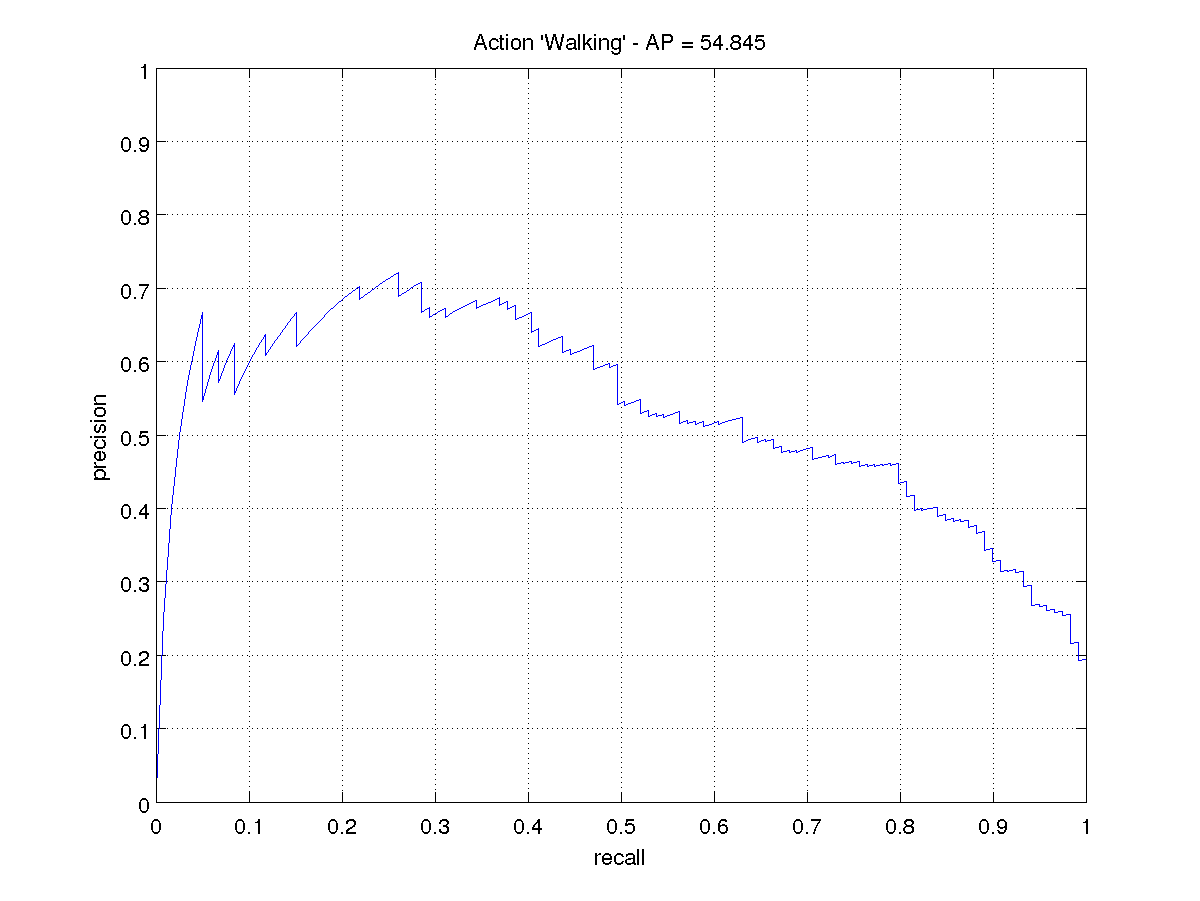
\includegraphics[height=5cm]{img/LSVM_PR_Walking.png}
\end{minipage}
\end{figure}

%\nocite{*}
%\bibliographystyle{splncs}
%\bibliography{biblio/references}


\end{document}













